\documentclass[empirical, authordate, issue]{jote-new-article}

\addbibresource{bibliography.bib}
\newrobustcmd{\B}{\DeclareFontSeriesDefault[rm]{bf}{b}\bfseries}

\begin{filecontents}{bibliography.bib}
 

    @article{Lewandowsky2017,
      title       = {Beyond Misinformation: Understanding and Coping with the “Post-Truth" Era},
      author      = {Lewandowsky, S. and Ecker, U. K. H. and Cook, J.},
      number      = {4},
      volume      = {6},
      url         = {https://doi.org/10.1016/j.jarmac.2017.07.008},
      doi         = {10.1016/j.jarmac.2017.07.008},
      year        = {2017},
      pages       = {353--369},
      journal     = {Era. Journal of Applied Research in Memory and Cognition}
  }
  
  
  @article{Arun2019,
      title       = {On {WhatsApp}, rumours, lynchings, and the {Indian} Government},
      author      = {Arun, C.},
      number      = {6},
      volume      = {54},
      url         = {https://papers.ssrn.com/sol3/papers.cfm?abstract\_id=3336127},
      year        = {2019},
      pages       = {30--35},
      journal     = {Economic \& Political Weekly}
  }
  
  
  @article{Sundar2021,
      title       = {Seeing is believing: Is video modality more powerful in spreading fake news via online messaging apps?},
      author      = {Sundar, S. S. and Molina, M. D. and Cho, E.},
      number      = {6},
      volume      = {26},
      url         = {https://doi.org/10.1093/jcmc/zmab010},
      doi         = {10.1093/jcmc/zmab010},
      year        = {2021},
      pages       = {301--319},
      journal     = {Journal of Computer-Mediated Communication}
  }
  
  
  @article{Vasudeva2020,
      title       = {{WhatsApp} in {India}? A case study of social media related lynchings},
      author      = {Vasudeva, F. and Barkdull, N.},
      number      = {5},
      volume      = {26},
      url         = {https://doi-org.ezp.lib.cam.ac.uk/10.1080/13504630.2020.1782730},
      year        = {2020},
      pages       = {574--589},
      journal     = {Social Identities}
  }
  
  
  @article{Banaji2019,
      title       = {{WhatsApp} Vigilantes: An exploration of citizen reception and circulation of {WhatsApp} misinformation linked to mob violence in {India}},
      author      = {Banaji, S. and Bhat, R. and Agarwal, A. and Passanha, N. and Sadhana Pravin, M.},
      url         = {http://eprints.lse.ac.uk/104316/},
      year        = {2019}
  }
  
  
  @article{Badrinathan2021,
      title       = {Educative Interventions to Combat Misinformation: Evidence From a Field Experiment in India},
      author      = {Badrinathan, S.},
      number      = {4},
      volume      = {115},
      url         = {https://doi.org/10.1017/S0003055421000459},
      doi         = {10.1017/S0003055421000459},
      year        = {2021},
      pages       = {1325--1341},
      journal     = {American Political Science Review}
  }
  
  
  @online{Mumo2021,
      title       = {Protecting Burundi's Vulnerable Media. Project Syndicate},
      author      = {Mumo, M.},
      url         = {https://www.project-syndicate.org/commentary/protecting-press-freedom-in-burundi-by-muthoki-mumo-2021-08},
      date        = {2021-08-25}
  }
  
  
  @article{Pasquetto2020,
      title       = {Understanding Misinformation on Mobile Instant Messengers (MIMs) in Developing Countries},
      author      = {Pasquetto, I.v and Center, S. and School, H. K. and Jahani, E. and Baranovsky, A. and Baum, M. A.},
      url         = {https://shorensteincenter.org/misinformation-on-mims/},
      year        = {2020}
  }
  
  
  @article{Reis2020,
      title       = {Can {WhatsApp} benefit from debunked fact-checked stories to reduce misinformation?},
      author      = {Reis, J. C. S. and Melo, P. and Garimella, K. and Benevenuto, F.},
      number      = {5},
      volume      = {1},
      url         = {https://doi.org/10.37016/mr-2020-035},
      doi         = {10.37016/mr-2020-035},
      year        = {2020},
      journal     = {Harvard Kennedy School Misinformation Review}
  }
  
  
  @article{Chibber2018,
      title       = {The Myth of Cote Buying in {India}},
      author      = {Chibber, K. P. and Verma, R.},
      publisher   = {Oxford Academic},
      year        = {2018},
      pages       = {103--130},
      journal     = {Ideology and Identity: The Changing Party Systems of {India}}
  }
  
  
  @article{Al-Zaman2021,
      title       = {A Thematic Analysis of Misinformation in {India} during the {COVID}-19 Pandemic},
      author      = {Al-Zaman, M. S.},
      url         = {https://doi.org/10.1080/10572317.2021.1908063},
      doi         = {10.1080/10572317.2021.1908063},
      year        = {2021},
      pages       = {1--11},
      journal     = {International Information and Library Review}
  }
  
  
  @article{Ferrara2020,
      title       = {What types of {COVID}-19 conspiracies are populated by Twitter bots?},
      author      = {Ferrara, E.},
      number      = {6},
      volume      = {25},
      url         = {https://doi.org/10.5210/fm.v25i6.10633},
      doi         = {10.5210/fm.v25i6.10633},
      year        = {2020},
      journal     = {First Monday}
  }
  
  
  @article{Henrich2010,
      title       = {The weirdest people in the world?},
      author      = {Henrich, J. and Heine, S. J. and Norenzayan, A.},
      number      = {2--3},
      volume      = {33},
      url         = {https://doi.org/10.1017/S0140525X0999152X},
      doi         = {10.1017/S0140525X0999152X},
      year        = {2010},
      pages       = {61--83},
      journal     = {Behavioral and Brain Sciences}
  }
  
  
  @article{Rad2018,
      title       = {Toward a psychology of Homo sapiens: Making psychological science more representative of the human population},
      author      = {Rad, M. S. and Martingano, A. J. and Ginges, J.},
      number      = {45},
      volume      = {115},
      url         = {https://doi.org/10.1073/pnas.1721165115},
      doi         = {10.1073/pnas.1721165115},
      year        = {2018},
      pages       = {11401--11405},
      journal     = {Proceedings of the National Academy of Sciences}
  }
  
  
  @article{Bhattacharjee2021,
      title       = {Internet Adoption in {India}},
      author      = {Bhattacharjee, B. and Pansari, S. and Dutta, A.},
      url         = {https://images.assettype.com/afaqs/2021-06/b9a3220f-ae2f-43db-a0b4-36a372b243c4/KANTAR\_ICUBE\_2020\_Report\_C1.pdf},
      year        = {2021}
  }
  
  
  @article{Kapoor2003,
      title       = {The relationship of individualism--collectivism and self-construals to communication styles in {India} and the {United States}},
      author      = {Kapoor, S. and Hughes, P. C. and Baldwin, J. R. and Blue, J.},
      number      = {6},
      volume      = {27},
      url         = {https://doi.org/10.1016/j.ijintrel.2003.08.002},
      doi         = {10.1016/j.ijintrel.2003.08.002},
      year        = {2003},
      pages       = {683--700},
      journal     = {International Journal of Intercultural Relations}
  }
  
  
  @article{Verma2020,
      title       = {The Measurement of Collectivism in {India}},
      author      = {Verma, J. and Triandis, H. C.},
      publisher   = {Swets \& Zeitlinger Publishers},
      year        = {2020},
      pages       = {256--265},
      journal     = {Merging Past, Present, and Future in Cross-Cultural Psychology: Selected papers from the Fourteenth International Congress of the International Association for Cross-Cultural Psychology}
  }
  
  
  @article{Rao2013,
      title       = {Globalization and the Identity Remix Among Urban Adolescents in {India}},
      author      = {Rao, M. A. and Berry, R. and Gonsalves, A. and Hastak, Y. and Shah, M. and Roeser, R. W.},
      number      = {1},
      volume      = {23},
      url         = {https://doi.org/10.1111/jora.12002},
      doi         = {10.1111/jora.12002},
      year        = {2013},
      pages       = {9--24},
      journal     = {Journal of Research on Adolescence}
  }
  
  
  @book{Vaishnav2019,
      title       = {The BJP in Power: {Indian} Democracy and Religious Nationalism},
      author      = {Vaishnav, M. and Jaffrelot, C. and Mehta, G. and Rej, A. and Shrinivasan, R. and Sagar, R. and Verma, R.},
      url         = {https://carnegieendowment.org/2019/04/04/bjp-in-power-indian-democracy-and-religious-nationalism-pub-78677},
      publisher   = {Carnegie Endowment for International Peace},
      year        = {2019}
  }
  
  
  @book{Campbell-Smith2019,
      title       = {Global Cyber Troops Country Profile: {India}},
      author      = {Campbell-Smith, U. and Bradshaw, S.},
      url         = {https://demtech.oii.ox.ac.uk/wp-content/uploads/sites/93/2019/05/India-Profile.pdf},
      publisher   = {Oxford Internet Institute, University of Oxford},
      year        = {2019}
  }
  
  
  @article{Ecker2022,
      title       = {The psychological drivers of misinformation belief and its resistance to correction},
      author      = {Ecker, U. K. H. and Lewandowsky, S. and Cook, J. and Schmid, P. and Fazio, L. K. and Brashier, N. and Kendeou, P. and Vraga, E. K. and Amazeen, M. A.},
      number      = {1},
      volume      = {1},
      url         = {https://doi.org/10.1038/s44159-021-00006-y},
      doi         = {10.1038/s44159-021-00006-y},
      year        = {2022},
      pages       = {13--29},
      journal     = {Nature Reviews Psychology}
  }
  
  
  @article{vanderLinden2022,
        doi = {10.1038/s41591-022-01713-6},
        url = {https://doi.org/10.1038/s41591-022-01713-6},
        year = 2022,
        month = {mar},
        publisher = {Springer Science and Business Media {LLC}},
        volume = {28},
        number = {3},
        pages = {460--467},
        author = {Sander van der Linden},
        title = {Misinformation: susceptibility, spread, and interventions to immunize the public},
  }

  @article{vanderLinden2017,
        doi = {10.1002/gch2.201600008},
        url = {https://doi.org/10.1002/gch2.201600008},
        year = 2017,
        month = {jan},
        publisher = {Wiley},
        volume = {1},
        number = {2},
        pages = {1600008},
        author = {Sander van der Linden and Anthony Leiserowitz and Seth Rosenthal and Edward Maibach},
        title = {Inoculating the Public against Misinformation about Climate Change},
        journal = {Global Challenges}
  }

@article{vanderLinden2017a,
        doi = {10.1126/science.aar4533},
        url = {https://doi.org/10.1126/science.aar4533},
        year = 2017,
        month = {dec},
        publisher = {American Association for the Advancement of Science ({AAAS})},
        volume = {358},
        number = {6367},
        pages = {1141--1142},
        author = {Sander van der Linden and Edward Maibach and John Cook and Anthony Leiserowitz and Stephan Lewandowsky},
        editor = {Jennifer Sills},
        title = {Inoculating against misinformation},
        journal = {Science} 
    }
  
  
  @article{Walter2018,
      title       = {How to unring the bell: A meta-analytic approach to correction of misinformation},
      author      = {Walter, N. and Murphy, S. T.},
      number      = {3},
      volume      = {85},
      url         = {https://doi.org/10.1080/03637751.2018.1467564},
      doi         = {10.1080/03637751.2018.1467564},
      year        = {2018},
      pages       = {423--441},
      journal     = {Communication Monographs}
  }
  
  
  @article{Clayton2020,
      title       = {Real Solutions for Fake News? Measuring the Effectiveness of General Warnings and Fact-Check Tags in Reducing Belief in False Stories on Social Media},
      author      = {Clayton, K. and Blair, S. and Busam, J. A. and Forstner, S. and Glance, J. and Green, G. and Kawata, A. and Kovvuri, A. and Martin, J. and Morgan, E. and Sandhu, M. and Sang, R. and Scholz-Bright, R. and Welch, A. T. and Wolff, A. G. and Zhou, A. and Nyhan, B.},
      number      = {4},
      volume      = {42},
      url         = {https://doi.org/10.1007/s11109-019-09533-0},
      doi         = {10.1007/s11109-019-09533-0},
      year        = {2020},
      pages       = {1073--1095},
      journal     = {Political Behavior}
  }
  
  
  @article{Porter2021,
      title       = {The global effectiveness of fact-checking: Evidence from simultaneous experiments in Argentina, Nigeria, South Africa, and the United Kingdom},
      author      = {Porter, E. and Wood, T. J.},
      number      = {37},
      volume      = {118},
      url         = {https://doi.org/10.1073/pnas.2104235118},
      doi         = {10.1073/pnas.2104235118},
      year        = {2021},
      pages       = {2104235118},
      journal     = {Proceedings of the National Academy of Sciences}
  }
  
  
  @article{Lewandowsky2012,
      title       = {Misinformation and Its Correction: Continued Influence and Successful Debiasing},
      author      = {Lewandowsky, S. and Ecker, U. K. H. and Seifert, C. M. and Schwarz, N. and Cook, J.},
      number      = {3},
      volume      = {13},
      url         = {https://doi.org/10.1177/1529100612451018},
      doi         = {10.1177/1529100612451018},
      year        = {2012},
      pages       = {106--131},
      journal     = {Psychological Science in the Public Interest}
  }
  
  
  @article{Walter2020,
      title       = {Fact-Checking: A Meta-Analysis of What Works and for Whom},
      author      = {Walter, N. and Cohen, J. and Holbert, R. L. and Morag, Y.},
      number      = {3},
      volume      = {37},
      url         = {https://doi.org/10.1080/10584609.2019.1668894},
      doi         = {10.1080/10584609.2019.1668894},
      year        = {2020},
      pages       = {350--375},
      journal     = {Political Communication}
  }
  
  
  @article{Pennycook2018,
      title       = {Prior exposure increases perceived accuracy of fake news},
      author      = {Pennycook, G. and Cannon, T. D. and Rand, D. G.},
      number      = {12},
      volume      = {147},
      url         = {https://doi.org/10.1037/xge0000465},
      doi         = {10.1037/xge0000465},
      year        = {2018},
      pages       = {1865--1880},
      journal     = {Journal of Experimental Psychology: General}
  }
  
  
  @article{Swire2017,
      title       = {The role of familiarity in correcting inaccurate information},
      author      = {Swire, B. and Ecker, U. K. H. and Lewandowsky, S.},
      number      = {12},
      volume      = {43},
      url         = {https://doi.org/10.1037/xlm0000422},
      doi         = {10.1037/xlm0000422},
      year        = {2017},
      pages       = {1948--1961},
      journal     = {Journal of Experimental Psychology: Learning, Memory, and Cognition}
  }
  
  
  @article{Roozenbeek2019,
      title       = {Fake news game confers psychological resistance against online misinformation},
      author      = {Roozenbeek, J. and van der Linden, S.},
      number      = {1},
      volume      = {5},
      url         = {https://doi.org/10.1057/s41599-019-0279-9},
      doi         = {10.1057/s41599-019-0279-9},
      year        = {2019},
      pages       = {65},
      journal     = {Palgrave Communications}
  }
  
  
  @article{Guess2020,
      title       = {A digital media literacy intervention increases discernment between mainstream and false news in the {United States} and {India}},
      author      = {Guess, A. M. and Lerner, M. and Lyons, B. and Montgomery, J. M. and Nyhan, B. and Reifler, J. and Sircar, N.},
      url         = {https://doi.org/10.1073/pnas.1920498117},
      doi         = {10.1073/pnas.1920498117},
      year        = {2020},
      pages       = {15536--15545},
      issue       = {27},
      volume      = {117},
      journal     = {Proceedings of the National Academy of Sciences of the {United States} of America}
  }
  
  
  @article{Bowles2020,
      title       = {Countering misinformation via {WhatsApp}: Preliminary evidence from the {COVID}-19 pandemic in Zimbabwe},
      author      = {Bowles, J. and Larreguy, H. and Liu, S.},
      number      = {10},
      volume      = {15},
      url         = {https://doi.org/10.1371/journal.pone.0240005},
      doi         = {10.1371/journal.pone.0240005},
      year        = {2020},
      pages       = {0240005},
      journal     = {PLoS ONE}
  }
  
  
  @article{Lewandowsky2021,
      title       = {Countering Misinformation and Fake News Through Inoculation and Prebunking},
      author      = {Lewandowsky, S. and van der Linden, S.},
      number      = {2},
      volume      = {32},
      url         = {https://doi.org/10.1080/10463283.2021.1876983},
      doi         = {10.1080/10463283.2021.1876983},
      year        = {2021},
      pages       = {348--384},
      journal     = {European Review of Social Psychology}
  }
  
  
  @article{McGuire1961,
      title       = {Resistance to persuasion conferred by active and passive prior refutation of the same and alternative counterarguments},
      author      = {McGuire, W. J.},
      number      = {2},
      volume      = {63},
      url         = {https://doi.org/10.1037/h0048344},
      doi         = {10.1037/h0048344},
      year        = {1961},
      pages       = {326--332},
      journal     = {The Journal of Abnormal and Social Psychology}
  }
  
  
  @article{McGuire1964,
      title       = {Some Contemporary Approaches},
      author      = {McGuire, W. J.},
      volume      = {1},
      url         = {https://doi.org/10.1016/S0065-2601(08)60052-0},
      doi         = {10.1016/S0065-2601(08)60052-0},
      publisher   = {Academic Press},
      year        = {1964},
      pages       = {191--229},
      journal     = {Advances in Experimental Social Psychology}
  }
  
  
  @inbook{Compton2012,
      title       = {Inoculation Theory},
      author      = {Compton, J.},
      publisher   = {Sage Publications, Inc},
      year        = {2012},
      pages       = {220--236},
      booktitle   = {The SAGE Handbook of Persuasion: Developments in Theory and Practice}
  }
  
  
  @article{Sagarin2002,
      title       = {Dispelling the illusion of invulnerability: The motivations and mechanisms of resistance to persuasion},
      author      = {Sagarin, B. J. and Cialdini, R. B. and Rice, W. E. and Serna, S. B.},
      number      = {3},
      volume      = {83},
      url         = {https://doi.org/10.1037/0022-3514.83.3.526},
      doi         = {10.1037/0022-3514.83.3.526},
      year        = {2002},
      pages       = {526--541},
      journal     = {Journal of Personality and Social Psychology}
  }
  
  
  @article{Banas2010,
      title       = {A Meta-Analysis of Research on Inoculation Theory},
      author      = {Banas, J. A. and Rains, S. A.},
      number      = {3},
      volume      = {77},
      url         = {https://doi.org/10.1080/03637751003758193},
      doi         = {10.1080/03637751003758193},
      year        = {2010},
      pages       = {281--311},
      journal     = {Communication Monographs}
  }
  
  
  @article{Compton2021,
      title       = {Threat and/in Inoculation Theory},
      author      = {Compton, J.},
      number      = {13},
      volume      = {15},
      url         = {https://ijoc.org/index.php/ijoc/article/view/17634},
      year        = {2021},
      pages       = {4294 -- 4307},
      journal     = {International Journal of Communication (Online}
  }

  @article{Compton2021a,
        doi = {10.1111/spc3.12602},
        url = {https://doi.org/10.1111/spc3.12602},
        year = 2021,
        month = {may},
        publisher = {Wiley},
        volume = {15},
        number = {6},
        author = {Josh Compton and Sander Linden and John Cook and Melisa Basol},
        title = {Inoculation theory in the post-truth era: Extant findings and new frontiers for contested science, misinformation, and conspiracy theories},
        journal = {Social and Personality Psychology Compass}
  }⏎                      
  
  
  @article{Roozenbeek2018,
      title       = {The fake news game: actively inoculating against the risk of misinformation},
      author      = {Roozenbeek, J. and van der Linden, S.},
      number      = {5},
      volume      = {22},
      url         = {https://doi.org/10.1080/13669877.2018.1443491},
      doi         = {10.1080/13669877.2018.1443491},
      year        = {2018},
      pages       = {570--580},
      journal     = {Journal of Risk Research}
  }
  
  
  @article{Banas2013,
      title       = {Inducing Resistance to Conspiracy Theory Propaganda: Testing Inoculation and Metainoculation Strategies},
      author      = {Banas, J. A. and Miller, G.},
      number      = {2},
      volume      = {39},
      url         = {https://doi.org/10.1111/hcre.12000},
      doi         = {10.1111/hcre.12000},
      year        = {2013},
      pages       = {184--207},
      journal     = {Human Communication Research}
  }
  
  
  @article{Jolley2017,
      title       = {Prevention is better than cure: Addressing anti-vaccine conspiracy theories},
      author      = {Jolley, D. and Douglas, K. M.},
      number      = {8},
      volume      = {47},
      url         = {https://doi.org/10.1111/jasp.12453},
      doi         = {10.1111/jasp.12453},
      year        = {2017},
      pages       = {459--469},
      journal     = {Journal of Applied Social Psychology}
  }
  
  
  @article{Cook2017,
      title       = {Neutralizing misinformation through inoculation: Exposing misleading argumentation techniques reduces their influence},
      author      = {Cook, J. and Lewandowsky, S. and Ecker, U. K. H.},
      number      = {5},
      volume      = {12},
      url         = {https://doi.org/10.1371/journal.pone.0175799},
      doi         = {10.1371/journal.pone.0175799},
      year        = {2017},
      pages       = {0175799},
      journal     = {PLOS ONE}
  }
  
  
  @article{Basol2020,
      title       = {Good News about Bad News: Gamified Inoculation Boosts Confidence and Cognitive Immunity Against Fake News},
      author      = {Basol, M. and Roozenbeek, J. and van der Linden, S.},
      number      = {1},
      volume      = {3},
      url         = {https://doi.org/10.5334/joc.91},
      doi         = {10.5334/joc.91},
      year        = {2020},
      pages       = {2},
      journal     = {Journal of Cognition}
  }
  
  
  @article{Maertens2021,
      title       = {Long-term effectiveness of inoculation against misinformation: Three longitudinal experiments},
      author      = {Maertens, R. and Roozenbeek, J. and Basol, M. and van der Linden, S.},
      number      = {1},
      volume      = {27},
      url         = {https://doi.org/10.1037/xap0000315},
      doi         = {10.1037/xap0000315},
      year        = {2021},
      pages       = {1--16},
      journal     = {Journal of Experimental Psychology: Applied}
  }
  
  
  @article{Bonetto2018,
      title       = {Priming Resistance to Persuasion decreases adherence to Conspiracy Theories},
      author      = {Bonetto, E. and Troïan, J. and Varet, F. and Monaco, G. and Girandola, F.},
      number      = {3},
      volume      = {13},
      url         = {https://doi.org/10.1080/15534510.2018.1471415},
      doi         = {10.1080/15534510.2018.1471415},
      year        = {2018},
      pages       = {125--136},
      journal     = {Social Influence}
  }
  
  
  @article{Roozenbeek2021,
      title       = {Disentangling Item and Testing Effects in Inoculation Research on Online Misinformation},
      author      = {Roozenbeek, J. and Maertens, R. and McClanahan, W. and van der Linden, S.},
      number      = {2},
      volume      = {81},
      url         = {https://doi.org/10.1177/0013164420940378},
      doi         = {10.1177/0013164420940378},
      year        = {2021},
      pages       = {340--362},
      journal     = {Solomon Revisited. Educational and Psychological Measurement}
  }
  
  
  @article{Basol2021,
      title       = {Towards psychological herd immunity: Cross-cultural evidence for two prebunking interventions against {COVID}-19 misinformation},
      author      = {Basol, M. and Roozenbeek, J. and Berriche, M. and Uenal, F. and McClanahan, W. P. and van der Linden, S.},
      number      = {1},
      volume      = {8},
      url         = {https://doi.org/10.1177/20539517211013868},
      doi         = {10.1177/20539517211013868},
      year        = {2021},
      pages       = {205395172110138},
      journal     = {Big Data \& Society}
  }
  
  
  @article{Pfau2005,
      title       = {Inoculation and Mental Processing: The Instrumental Role of Associative Networks in the Process of Resistance to Counterattitudinal Influence},
      author      = {Pfau, M. and Ivanov, B. and Houston, B. and Haigh, M. and Sims, J. and Gilchrist, E. and Russell, J. and Wigley, S. and Eckstein, J. and Richert, N.},
      number      = {4},
      volume      = {72},
      url         = {https://doi.org/10.1080/03637750500322578},
      doi         = {10.1080/03637750500322578},
      year        = {2005},
      pages       = {414--441},
      journal     = {Communication Monographs}
  }
  
  
  @article{Roozenbeek2020,
      title       = {Breaking Harmony Square: A game that “inoculates” against political misinformation},
      author      = {Roozenbeek, J. and van der Linden, S.},
      number      = {8},
      volume      = {1},
      url         = {https://doi.org/10.37016/mr-2020-4},
      doi         = {10.37016/mr-2020-4},
      year        = {2020},
      journal     = {The Harvard Kennedy School (HKS) Misinformation Review}
  }
  
  
  @inproceedings{Goga2015,
      title       = {The doppelgänger bot attack: Exploring identity impersonation in online social networks},
      author      = {Goga, O. and Venkatadri, G. and Gummadi, K. P.},
      url         = {https://doi.org/10.1145/2815675.2815699},
      doi         = {10.1145/2815675.2815699},
      place       = {IMC, Tokyo, Japan},
      date        = {2015-10-28/2015-10-30},
      pages       = {141--153},
      booktitle = {Proceedings of the ACM SIGCOMM Internet Measurement Conference}
  }
  
  
  @article{Jung2011,
      title       = {Twittering Away the Right of Publicity: Personality Rights and Twittering Away the Right of Publicity: Personality Rights and Celebrity Impersonation on Social Networking Websites},
      author      = {Jung, A. M.},
      number      = {1},
      volume      = {86},
      url         = {https://scholarship.kentlaw.iit.edu/cklawreview/vol86/iss1/16},
      year        = {2011},
      journal     = {Symposium on Energy Law Article}
  }
  
  
  @article{Reznik2013,
      title       = {Identity Theft on Social Networking Sites: Developing Issues of Internet Impersonation},
      author      = {Reznik, M.},
      number      = {2},
      volume      = {29},
      url         = {https://digitalcommons.tourolaw.edu/lawreviewAvailableat:https://digitalcommons.tourolaw.edu/lawreview/vol29/iss2/12https://digitalcommons.tourolaw.edu/lawreview/vol29/iss2/12},
      year        = {2013},
      pages       = {455--483},
      journal     = {Touro Law Review}
  }
  
  
  @article{Gross2004,
      title       = {Framing Emotional Response},
      author      = {Gross, K. and Ambrosio, L. D.},
      number      = {1},
      volume      = {25},
      url         = {https://www.jstor.org/stable/3792521},
      year        = {2004},
      pages       = {1--29},
      journal     = {Political Psychology}
  }
  
  
  @inbook{Konijn2012,
      title       = {The Role of Emotion in Media Use and Effects},
      author      = {Konijn, E. A.},
      publisher   = {Oxford University Press},
      year        = {2012},
      pages       = {186--211},
      booktitle = {The Oxford Handbook of Media Psychology}
  }
  
  
  @article{Zollo2015,
      title       = {Emotional dynamics in the age of misinformation},
      author      = {Zollo, F. and Novak, P. K. and Vicario, M. and Bessi, A. and Mozetič, I. and Scala, A. and Caldarelli, G. and Quattrociocchi, W. and Preis, T.},
      number      = {9},
      volume      = {10},
      url         = {https://doi.org/10.1371/journal.pone.0138740},
      doi         = {10.1371/journal.pone.0138740},
      year        = {2015},
      pages       = {0138740},
      journal     = {PLoS ONE}
  }
  
  
  @article{Groenendyk2018,
      title       = {Competing Motives in a Polarized Electorate: Political Responsiveness, Identity Defensiveness, and the Rise of Partisan Antipathy},
      author      = {Groenendyk, E.},
      number      = {S1},
      volume      = {39},
      url         = {https://doi.org/10.1111/pops.12481},
      doi         = {10.1111/pops.12481},
      year        = {2018},
      pages       = {159--171},
      journal     = {Political Psychology}
  }
  
  
  @article{Iyengar2018,
      title       = {The Strengthening of Partisan Affect},
      author      = {Iyengar, S. and Krupenkin, M.},
      volume      = {39},
      url         = {https://doi.org/10.1111/pops.12487},
      doi         = {10.1111/pops.12487},
      year        = {2018},
      pages       = {201--218},
      journal     = {Political Psychology}
  }
  
  
  @online{BBCMonitoring2021,
      title       = {Israel-Palestinian conflict: False and misleading claims fact-checked},
      author      = {{BBC Monitoring}},
      url         = {https://www.bbc.co.uk/news/57111293},
      date        = {2021-05-16},
      journal     = {BBC News}
  }
  
  
  @article{Robb2021,
      title       = {Anatomy of a Fake News Scandal. Rolling Stone},
      author      = {Robb, A.},
      url         = {https://www.rollingstone.com/feature/anatomy-of-a-fake-news-scandal-125877/},
      date        = {2021-11-16}
  }
  
  
  @online{McLaughlin2018,
      title       = {How {WhatsApp} Fuels Fake News and Violence in {India}},
      author      = {McLaughlin, T.},
      url         = {https://www.wired.com/story/how-whatsapp-fuels-fake-news-and-violence-in-india/},
      date        = {2018-12-12}
  }
  
  
  @online{Findlay2019,
      title       = {{WhatsApp} says {Indian} rules on encryption ‘not possible' to meet},
      author      = {Findlay, S.},
      url         = {https://www.ft.com/content/9fcfa604-2a0d-11e9-88a4-c32129756dd8},
      date        = {2019-02-06},
      journal     = {Financial Times}
  }
  
  
  @report{Park2013,
      title       = {British Social Attitudes: the 30th Report},
      author      = {Park, A. and Bryson, C. and Clery, E. and Curtice, J. and Philips, M.},
      publisher   = {NatCen Social Research},
      year        = {2013},
      url         = {https://www.bsa.natcen.ac.uk/latest-report/british-social-attitudes-30/key-findings/introduction.aspx}
  }
  
  
  @article{Adewole2017,
      title       = {Malicious accounts: Dark of the social networks},
      author      = {Adewole, K. S. and Anuar, N. B. and Kamsin, A. and Varathan, K. D. and Razak, S. A.},
      volume      = {79},
      url         = {https://doi.org/10.1016/j.jnca.2016.11.030},
      doi         = {10.1016/j.jnca.2016.11.030},
      year        = {2017},
      pages       = {41--67},
      journal     = {Journal of Network and Computer Applications}
  }
  
  
  @article{Rathje2021,
      title       = {Out-group animosity drives engagement on social media. Proceedings of the National Academy of Sciences, 118(26},
      author      = {Rathje, S. and Bavel, J. J. and van der Linden, S.},
      url         = {https://doi.org/10.1073/pnas.2024292118},
      doi         = {10.1073/pnas.2024292118},
      year        = {2021},
      pages       = {2024292118}
  }
  
  
  @article{Melki2014,
      title       = {Ideological polarization and the media},
      author      = {Melki, M. and Pickering, A.},
      number      = {1},
      volume      = {125},
      url         = {https://doi.org/10.1016/j.econlet.2014.08.008},
      doi         = {10.1016/j.econlet.2014.08.008},
      year        = {2014},
      pages       = {36--39},
      journal     = {Economics Letters}
  }
  
  
  @article{Lakens2018,
      title       = {Equivalence Testing for Psychological Research: A Tutorial},
      author      = {Lakens, D. and Scheel, A. M. and Isager, P. M.},
      number      = {2},
      volume      = {1},
      url         = {https://doi.org/10.1177/2515245918770963},
      doi         = {10.1177/2515245918770963},
      year        = {2018},
      pages       = {259--269},
      journal     = {Advances in Methods and Practices in Psychological Science}
  }
  
  
  @article{Dienes2014,
      title       = {Using Bayes to get the most out of non-significant results},
      author      = {Dienes, Z.},
      volume      = {5},
      url         = {https://doi.org/10.3389/fpsyg.2014.00781},
      doi         = {10.3389/fpsyg.2014.00781},
      year        = {2014},
      pages       = {781},
      journal     = {Frontiers in Psychology}
  }
  
  
  @article{Iyengar2022,
      title       = {Inoculation against conspiracy theories: A consumer side approach to {India}'s fake news problem},
      author      = {Iyengar, A. and Gupta, P. and Priya, N.},
      url         = {https://doi.org/},
      doi         = {10.1002/acp.3995},
      year        = {2022},
      journal     = {Applied Cognitive Psychology}
  }
  
  
  @article{Basol2022,
      title       = {Gamified inoculation against misinformation on {WhatsApp}},
      author      = {Basol, M. and Roozenbeek, J. and van der Linden, S.},
      publisher   = {Department of Psychology, University of Cambridge},
      date        = {2022-05-19}
  }
  
  
  @article{Traberg2022,
      title       = {Psychological inoculation against misinformation: Current Evidence and Future Directions},
      author      = {Traberg, C. and Roozenbeek, J. and van der Linden, S.},
      volume      = {700},
      year        = {2022},
      journal     = {The ANNALS of the American Academy of Political and Social Science}
  }
  
  
  @article{Medeiros2021,
      title       = {Addressing misinformation on {WhatsApp} in {India} through intermediary liability policy, platform design modification, and media literacy},
      author      = {Medeiros, B. and Singh, P.},
      volume      = {10},
      url         = {https://doi.org/10.5325/JINFOPOLI.10.2020.0276},
      doi         = {10.5325/JINFOPOLI.10.2020.0276},
      publisher   = {Penn State University Press},
      year        = {2021},
      pages       = {276--298},
      journal     = {Journal of Information Policy}
  }
  
  
  @article{Ivanov2022,
      title       = {The Role of Threat and Counterarguing in Therapeutic Inoculation},
      author      = {Ivanov, B. and Rains, S. A. and Dillingham, L. L. and Parker, K. A. and Geegan, S. A. and Barbati, J. L.},
      number      = {1},
      volume      = {87},
      url         = {https://doi.org/10.1080/1041794X.2021.1983012},
      doi         = {10.1080/1041794X.2021.1983012},
      year        = {2022},
      pages       = {15--27},
      journal     = {Southern Communication Journal}
  }
  
  
  @article{Wood2007,
      title       = {Rethinking the Inoculation Analogy: Effects on Subjects With Differing Preexisting Attitudes},
      author      = {Wood, M. L. M.},
      number      = {3},
      volume      = {33},
      url         = {https://doi.org/10.1111/j.1468-2958.2007.00303.x},
      doi         = {10.1111/j.1468-2958.2007.00303.x},
      year        = {2007},
      pages       = {357--378},
      journal     = {Human Communication Research}
  }
  
  
  @article{Banas2017,
      title       = {Apprehension or motivation to defend attitudes? Exploring the underlying threat mechanism in inoculation-induced resistance to persuasion},
      author      = {Banas, J. A. and Richards, A. S.},
      number      = {2},
      volume      = {84},
      url         = {https://doi.org/10.1080/03637751.2017.1307999},
      doi         = {10.1080/03637751.2017.1307999},
      year        = {2017},
      pages       = {164--178},
      journal     = {Communication Monographs}
  }
  
  
  @article{Kwan2016,
      title       = {Anger and perception of unfairness and harm: Cultural differences in normative processes that justify sanction assignment},
      author      = {Kwan, L. Y.-Y.},
      number      = {1},
      volume      = {19},
      url         = {https://doi.org/10.1111/ajsp.12119},
      doi         = {10.1111/ajsp.12119},
      year        = {2016},
      pages       = {6--15},
      journal     = {Asian Journal of Social Psychology}
  }
  
  
  @article{Lim2004,
      title       = {Cross Cultural Differences in Online Learning Motivation},
      author      = {Lim, D. H.},
      number      = {2},
      volume      = {41},
      url         = {https://doi.org/10.1080/09523980410001685784},
      doi         = {10.1080/09523980410001685784},
      year        = {2004},
      pages       = {163--175},
      journal     = {Educational Media International}
  }
  
  
  @article{Matsumoto2008,
      title       = {Culture, emotion regulation, and adjustment},
      author      = {Matsumoto, D. and Yoo, S. H. and Nakagawa, S.},
      number      = {6},
      volume      = {94},
      url         = {https://doi.org/10.1037/0022-3514.94.6.925},
      doi         = {10.1037/0022-3514.94.6.925},
      year        = {2008},
      pages       = {925--937},
      journal     = {Journal of Personality and Social Psychology}
  }
  
  
  @article{Mesquita2003,
      title       = {Cultural differences in emotions: a context for interpreting emotional experiences},
      author      = {Mesquita, B. and Walker, R.},
      number      = {7},
      volume      = {41},
      url         = {https://doi.org/10.1016/S0005-7967(02)00189-4},
      doi         = {10.1016/S0005-7967(02)00189-4},
      year        = {2003},
      pages       = {777--793},
      journal     = {Behaviour Research and Therapy}
  }
  
  
  @article{EncyclopaediaBritannica2012,
      title       = {Santhal},
      author      = {{The Editors of Encyclopaedia Britannica}},
      url         = {https://www.britannica.com/topic/Santhal},
      date        = {2012-07-19},
      journal     = {{Encyclopaedia Britannica}}
  }
  
  
  @online{India2016,
      title       = {Rural and Urban Composition of Population -- Census 2011 and 2011},
      author      = {{Government of India}},
      url         = {https://data.gov.in/resource/rural-and-urban-composition-population-census-2001-and-2011},
      year        = {2016}
  }
  
  
  @article{Shahid2022,
      title       = {Examining Source Effects Perceptions of Fake News in {India}},
      author      = {Shahid, F. and Mare, S. and Vashistha, A.},
      number      = {CSW1, 89},
      volume      = {6},
      url         = {https://doi.org/10.1145/3512936},
      doi         = {10.1145/3512936},
      year        = {2022},
      pages       = {1--29},
      journal     = {Proceedings of the ACM on Human-Computer Interaction}
  }
  
  
  @online{Mothkoor2021,
      title       = {The digital dream: Upskilling {India} for the future},
      author      = {Mothkoor, V. and Mumtaz, F.},
      url         = {https://www.ideasforindia.in/topics/governance/the-digital-dream-upskilling-india-for-the-future.html\#:\textasciitilde{}:text=Digital\%20literacy\%20levels\%20in\%20India\&text=Based\%20on\%20the\%20above\%20definition,just\%2025\%25\%20in\%20rural\%20areas.},
      date        = {2021-03-23}
  }
  
  
  @article{Rowntree2020,
      title       = {The Mobile Gender Gap Report 2020},
      author      = {Rowntree, O. and Shahnan, M. and Bahia, K. and Butler, C. and Lindsey, D. and Sibthorpe, C.},
      url         = {https://www.gsma.com/mobilefordevelopment/wp-content/uploads/2020/05/GSMA-The-Mobile-Gender-Gap-Report-2020.pdf},
      year        = {2020}
  }
  
  
  @article{Pogorelskiy2017,
      title       = {News Sharing and Voting on Social Networks: An Experimental Study},
      author      = {Pogorelskiy, K. and Shum, M.},
      url         = {https://doi.org/10.2139/ssrn.2972231},
      doi         = {10.2139/ssrn.2972231},
      year        = {2017},
      journal     = {SSRN Electronic Journal}
  }
  
  
  @article{Sircar2019,
      title       = {Dilemmas and Challenges of Citizen Information Campaigns: Lessons from a Failed Experiment in {India}},
      author      = {Sircar, N. and Chauchard, S.},
      url         = {https://doi.org/10.1017/9781108381390.011},
      doi         = {10.1017/9781108381390.011},
      publisher   = {Cambridge University Press},
      year        = {2019},
      pages       = {287--312},
      journal     = {Information, Accountability, and Cumulative Learning}
  }
  
  
  @article{Deshmukh2019,
      title       = {Methodological issues and Problems of Conducting Surveys in {India}. A Commentary by the {Indian} ISSP Partner Organization},
      author      = {Deshmukh, Y.},
      number      = {5-6},
      volume      = {49},
      url         = {https://doi.org/10.1080/00207659.2019.1683286},
      doi         = {10.1080/00207659.2019.1683286},
      year        = {2019},
      pages       = {400--411},
      journal     = {International Journal of Sociology}
  }
  
  
  @article{Ghai2021,
      title       = {It's time to reimagine sample diversity and retire the WEIRD dichotomy},
      author      = {Ghai, S.},
      number      = {8},
      volume      = {5},
      url         = {https://doi.org/10.1038/s41562-021-01175-9},
      doi         = {10.1038/s41562-021-01175-9},
      year        = {2021},
      pages       = {971--972},
      journal     = {Nature Human Behaviour}
  }
  
  \end{filecontents}
  
\jotetitle{Gamified Inoculation Against Misinformation in India: \mbox{A Randomized Control Trial} }
\keywordsabstract{misinformation, India, inoculation theory, pre-bunking, \mbox{WhatsApp}}
\abstracttext{Although the spread of misinformation is a pervasive and disruptive global problem, extant research is skewed towards “WEIRD” countries leaving questions about how to tackle misinformation in the developing world with different media and consumption patterns unanswered. We report the results of a game-based intervention against misinformation in India. The game is based on the mechanism of psychological inoculation; borrowed from the medical context, inoculation interventions aim to pre-emptively neutralize falsehoods and help audiences spot and resist misinformation strategies. Though the efficacy of these games has been repeatedly demonstrated in samples from Western countries, the present study conducted in north India (\emph{n} = 757) did not replicate earlier findings. We found no significant impact of the intervention on the perceived reliability of messages containing misinformation, confidence judgments, and willingness to share information with others. Our experience presents a teachable moment for the unique challenges associated with complex cultural adaptations and field work in rural areas. These results have significant ramifications for designing misinformation interventions in developing countries where misinformation is largely spread via encrypted messaging applications such as \mbox{WhatsApp}. Our findings contribute to the small but growing body of work looking at how to adapt misinformation interventions to cross-cultural settings.}
\runningauthor{Harjani et al.}
\jname{Journal of Trial \& Error}
\funding{}
\paperdoi{10.36850/e12}
\paperreceived{June 7, 2022}
\author[1]{Trisha Harjani\orcid{https://orcid.org/0000-0002-5829-9485}}
\authortwo{Trisha Harjani}
\affil[1]{University of Cambridge}
\corremail{\href{mailto:th649@cam.ac.uk}{th649@cam.ac.uk}}
\corraddress{University of Cambridge}
\author[1]{Melisa-Sinem Basol\orcid{https://orcid.org/0000-0003-1480-6462}}
\authorthree{Melisa-Sinem Basol}
\author[1]{Jon  Roozenbeek\orcid{https://orcid.org/0000-0002-8150-9305}}
\authorfour{Jon  Roozenbeek}
\author[1]{Sander  van der Linden \orcid{https://orcid.org/0000-0002-0269-1744}}
\authorfive{Sander  van der Linden }
\paperaccepted{October 10, 2022}
\jwebsite{https://journal.trialanderror.org}
\jyear{2023}
\paperpublished{February 27, 2023}
\paperpublisheddate{2023-02-27}

\acknowledgments{We would like to thank our partners Digital Empowerment Foundation in India for implementing the survey and \mbox{WhatsApp}/Meta for funding.}
\DeclareCaptionLabelFormat{supplement}{
    \textbf{#1 S#2}
}

\jvolume{3}
\jissue{1}
\paperissued{December 31, 2023}
\jpages{14--56}

\begin{document}

\setcounter{page}{14}

\begin{frontmatter}
  \maketitle

  \begin{abstract}
    \printabstracttext
  \end{abstract}
\end{frontmatter}





















\lettrine{T}{he} spread of misinformation online is widely documented as a threat to democracies worldwide \parencite{Lewandowsky2017, vanderLinden2017a}. In India, the world's largest democracy, the sharing of misinformation online has been linked to mob violence, and even killings \parencite{Arun2019, Sundar2021, Vasudeva2020}. While social media platforms such as Facebook or Twitter can flag misinformed content or remove it from their platforms, mobile instant messenger services such as \mbox{WhatsApp} and Telegram are limited by their end-to-end encrypted nature \parencite{Banaji2019}. Private conversations or groups form a closed network where misinformation can freely circulate without monitoring and studies have shown that this takes place in India \parencite{Badrinathan2021}, as well as Burundi \parencite{Mumo2021}, Nigeria, Brazil, and Pakistan \parencite{Pasquetto2020}. Furthermore, a significant proportion of the misinformation shared in India continues to be shared and circulated on \mbox{WhatsApp} even after being falsified by professional, third-party fact checkers \parencite{Reis2020}. This trend has created a breeding ground for unverified, misleading, or false information, some of which originates from political parties \parencite{Chibber2018}. Despite \mbox{WhatsApp}'s countermeasures, which include implementing digital literacy programs, placing restrictions on forwarding, and broadcasting awareness-raising adverts, misinformation on the platform is persistent and has been exacerbated by COVID-19 \parencite{Al-Zaman2021, Ferrara2020}. Given the limitations of implementing algorithmic solutions on private messaging platforms \parencite{Reis2020}, user-level solutions are an increasingly important avenue of research.

The overwhelming majority of individual-level misinformation interventions have been tested on populations from developed, Western countries. This is indeed a feature of behavioral science in general where non-WEIRD (western, educated, industrialized, rich and democratic) samples are underrepresented \parencite{Henrich2010, Rad2018}. There are several factors that could impede the generalizability of findings to India specifically. Since 2017, year-on-year internet penetration in India has grown by 13\% in rural areas compared to 4\% in urban neighborhoods \parencite{Bhattacharjee2021}. While misinformation can be spread by both urban and rural residents, the latter are likely to access the internet via 2G networks with limited resources for fact checking and a tendency to distribute \mbox{WhatsApp} messages with low reflexivity, as a mode of group participation or strategy to avoid feelings of exclusion \parencite{Banaji2019}. Given the collectivist culture in India \parencite{Kapoor2003, Verma2020}, even amongst youth samples \parencite{Rao2013}, the importance of group identities is heightened. Political parties frequently capitalize on these divisions, often along religious lines \parencite{Vaishnav2019}. Furthermore, the institutionalization of misinformation dissemination by political parties in India, whereby ‘IT cells' troll and spread automated content, is not uncommon \parencite{Campbell-Smith2019} as part of their campaigning strategy \parencite{Banaji2019}.

\begin{takeHomeMessage}

  This study found that gamified inoculation interventions, which have worked well in Western countries, did not confer psychological resistance against misinformation to participants in India. This null result (possibly due to lower digital literacy rates) calls for further investigation into bottom-up interventions tackling misinformation on messaging platforms in developing countries.
\end{takeHomeMessage}





To counter the spread of misinformation, several strategies have been researched at the individual level, the most well-known of which include fact-checking and “debunking” or correcting false information after exposure \parencite{Ecker2022, vanderLinden2022, Walter2018}. Studies examining the efficacy of such corrective measures have revealed mixed results. Although some have found that fact-checking can improve accuracy assessments \parencite{Clayton2020, Porter2021, Walter2018}, there are several drawbacks to correcting misinformation post-exposure. One major issue concerns the continued influence of misinformation or the tendency for people to continue making inferences based on misinformation. They do so even when they acknowledge a correction \parencite{Ecker2022, Lewandowsky2012}, which limits the correction's potential effectiveness. This is further compounded by the finding that (a) not all audiences are receptive to fact-checks \parencite{Walter2020}, (b) repeated exposure to misinformation can increase its perceived accuracy \parencite{Pennycook2018, Swire2017}, and (c) that corrections do not scale, meaning they rarely reach the same number people as the initial misinformation \parencite{Roozenbeek2019, vanderLinden2022}. Lastly, corrective strategies are also difficult to implement on private messaging platforms given the invisibility of information flow in this sphere \parencite{Reis2020}.

Accordingly, studies which have evaluated fact-checking and literacy interventions in developing countries have revealed inconclusive results. For example, \textcite{Guess2020} tested the effect of providing U. S. and Indian participants with tips on how to spot misinformation. They found a positive impact on people's ability to detect false information in the U. S. and in a highly educated online Indian sample, but not in a face-to-face sample obtained in rural Northern India. Similarly, \textcite{Badrinathan2021} tested the impact of an intensive one-hour in-person media literacy training during the 2019 national election and found no significant beneficial effects.

One study tested the impact of a debunking intervention via \mbox{WhatsApp} broadcast messaging in Zimbabwe, another country with high \mbox{WhatsApp} usage, finding that participants had increased knowledge about COVID-19 \parencite{Bowles2020}. \textcite{Pasquetto2020} further found that, while corrections on encrypted group chats reduced belief in misinformation in India and Pakistan, \mbox{WhatsApp} users report corrections as unusual and socially awkward. Given the known challenges surrounding debunking and fact-checking, a promising effort against misinformation has been to pre-emptively debunk (or \emph{prebunk}) falsehoods to allow individuals to acquire skills to detect and resist misinformation in the future \parencite{Lewandowsky2021}. This approach is based on the theory of psychological inoculation \parencite{McGuire1961}.

\section{Theoretical Background: Prebunking and Inoculation Theory}

Inoculation theory was originally developed in the 1960s and is based on the biological process of immunization \parencite{McGuire1964, McGuire1961}: just as exposure to a weakened dose of a pathogen can confer immunity against future infection(s), pre-emptively exposing people to weakened doses of misinformation—along with strong refutations—can cultivate cognitive immunity to future manipulation attempts. Inoculation theory has two key components. Firstly, the inoculation must have a forewarning to evoke threat or the motivation for people to defend themselves from a potential attack on their attitudes \parencite{Compton2012}. Being aware of one's vulnerability to manipulation is important for kick-starting resistance to persuasion \parencite{Sagarin2002}. Secondly, much like the injection of a weakened dose of a virus can build immunity through the production of antibodies, exposure to a weakened version of a persuasive argument along with a counterargument can inspire lowered vulnerability to misleading persuasion attempts \parencite{McGuire1961}. A meta-analysis of inoculation theory has found that it is effective at building resistance against persuasion across issues \parencite{Banas2010}.

In more recent years, the theory has informed the design of inoculation interventions aiming to endow attitudinal resistance against online misinformation specifically \parencite[for in-depth reviews see][]{Compton2021a, Lewandowsky2021, Roozenbeek2018, vanderLinden2022}. Some recent applications of inoculation theory include even potentially polarizing topics such as climate change \parencite{vanderLinden2017}, conspiracy theories \parencite{Banas2013}, or vaccinations \parencite{Jolley2017}. However, all these studies aimed to inoculate people against misinformation about a specific issue. As such, they do not necessarily imply that the inoculation would be effective as a “broad-spectrum vaccine” against misinformation \parencite{Roozenbeek2018}. This prompted a shift away from narrow-spectrum inoculations to those that incorporate persuasion techniques common to misinformation more generally \parencite{Cook2017, Roozenbeek2019}. In other words, familiarity with a weakened dose of the underlying \emph{techniques} that are used to spread misinformation could impart an increased cognitive ability to detect manipulative information that makes use of such misinformation tactics. These tactics include emotionally manipulative language, group polarization, conspiratorial reasoning, trolling, and impersonations of fake experts, politicians, and celebrities \parencite{Roozenbeek2019}.

This strategy has demonstrated fairly consistent success \parencite{Basol2020, Cook2017, Roozenbeek2019} including long-term efficacy, provided inoculated individuals are given short reminders or “booster shots” of the lessons learned \parencite{Maertens2021}. Yet, no study to date has tested the effect of inoculation interventions on the Indian population and inoculation researchers have noted a lack of generalizability of inoculation scholarship to non-WEIRD populations \parencite{Bonetto2018}, demanding interventions be adapted and evaluated.

\section{Recent Applications: Inoculation Games}

Recent applications of inoculation theory also depart from the traditional method of providing participants with ready-made counterarguments (so-called “passive inoculation”) and instead use an “active” form of inoculation whereby participants themselves\textbf{ }play an active role in generating resistance to manipulation \parencite{Roozenbeek2018}. Gamified interventions have proven to be a fruitful vehicle for active inoculation. One example of such an inoculation intervention is the online game \emph{Bad News }(www.getbadnews.com): in this game, players find themselves in an artificial social media environment designed to mimic the features of widely used online platforms \parencite{Basol2020, Maertens2021, Roozenbeek2021, Roozenbeek2019}. Across six levels, players are warned about the dangers of fake news, and they develop an understanding of several widely used misinformation techniques through exposure to weakened dose of these tactics alongside ways to spot them. Evidence for the relative benefits of “active” inoculation is emerging \parencite{Basol2021}, particularly because it may strengthen associative memory networks, contributing towards higher resistance to persuasion \parencite{Pfau2005}.

However, the \emph{Bad News }game, as well as two others \parencite[\emph{Harmony Square}][]{Roozenbeek2020} and \parencite[\emph{Go Viral!}][]{Basol2021}, all focus on misinformation on public social media platforms (such as Facebook and Twitter). This reduces the potential applicability of these games in countries where direct messaging apps are a more common means of communication than public social media platforms. To address this problem, we engaged in a novel real-world collaboration with \mbox{WhatsApp}, Inc (Meta platforms) and developed a new game that inoculates people against misinformation on direct messaging apps, called \emph{Join this Group }(link to English version; \url{https://whatsapp.aboutbadnews.com}). The Hindi-version of the game was tested in this study (further details in the method section). Its purpose is to inoculate participants against four manipulation techniques commonly present in misinformation on direct messaging apps. Specifically, these techniques are the impersonation of a fake expert \parencite{Goga2015, Jung2011, Reznik2013}, use of emotional language to frame content \parencite{Gross2004, Konijn2012, Zollo2015}, polarization of narratives to create hostility towards the opposition \parencite{Groenendyk2018, Iyengar2018}, and the escalation of an issue such that misinformation triggers offline acts of aggression \parencite{BBCMonitoring2021, Robb2021}.



\section{The Present Research}

This paper seeks to address two gaps in the literature on misinformation interventions. We first aim to understand whether inoculation against misinformation can improve people's ability to spot misinformation that is commonly shared in a private messaging context (such as on \mbox{WhatsApp}). Second, our sample is from India, an understudied population where the spread of misinformation via private messaging platforms has been linked to violence \parencite{McLaughlin2018}. We ran a field experiment in India testing the efficacy of the inoculation game, \emph{Join this Group}.\textbf{ }

This paper therefore makes two unique advancements to the literature. This study is the first to test an inoculation intervention against misinformation shared in the context of private messaging. This domain of information exchange is markedly different to public platforms such that the burden of identifying, addressing, and correcting misinformation falls on the user(s) \parencite{Pasquetto2020}. Moreover, we test the effectiveness of these modified interventions in India (\emph{n} = 757), the largest market for \mbox{WhatsApp} globally \parencite{Findlay2019}. Both studies were approved by the Cambridge Psychology Research Ethics Committee (REC-2018-19/19). [Data and scripts are deposited on the Open Science Framework: https://osf.io/abjrg].

\section{Method}

We conducted a 2 (treatment -- control) x 2 (pre -- post) mixed-between randomized control trial on a sample collected from 8 North Indian states (Bihar, Chhattisgarh, Haryana, Jharkhand, Madhya Pradesh, Rajasthan, Uttar Pradesh, and National Capital Territory (Delhi)). Participants were recruited as part of media literacy workshops administered to 1283 individuals. The experiment was conducted door-to-door, in person, with the assistance of iPads and smartphones through which participants could access the online intervention. After providing informed consent, participants were asked to indicate their frequency of \mbox{WhatsApp} usage in the last twelve months on a 5-point scale, ranging from “\emph{Never”} to “\emph{More than once a day}”. Participants were then shown 16 screenshots of \mbox{WhatsApp} conversations in a randomized order (see Figure \ref{fig:figure1}) and, following \textcite{Roozenbeek2021}, were asked to make three assessments: how reliable they found the post (1), how confident they are in their reliability assessment (2) and how likely they would be to share the message (3). All three assessments were rated on a 1-7 Likert scale (1 being “\emph{Not at all”}, 4 being “\emph{Neutral}”, and 7 being “\emph{Very much}”). Of the 16 images, four were screenshots of authentic \mbox{WhatsApp} conversations, of which two were fake news and two contained accurate information. The remaining 12 were screenshots containing misinformation designed to demonstrate four manipulation techniques (fake expert, emotion, polarization, and escalation). The four real (non-misinformation) items were sourced from fact-checking websites and the manipulative items were created by one of the authors and validated by two other authors, to ensure that the conversations make appropriate use of a misinformation technique. Figure~\ref{fig:figure1} demonstrates an example of eliciting fear using emotional language in misinformation messaging.

\begin{figure}

  \begin{fullwidth}
    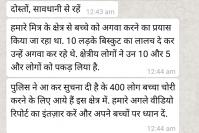
\includegraphics[width=\linewidth]{media/image1.jpeg}
    \caption{\mbox{WhatsApp} messages containing emotional misinformation messaging. This image is an example of one used in the experimental pre-test and post-test measure. The screenshot reads: “Friends, be careful”, “Attempts are being made to kidnap a child from our friend's area. 10 boys were kidnapping him with the promise of biscuits. People in the area have caught those 10 and 5 more people”, “The police has announced that 400 people had come to steal the child in this area. Wait for our next video that will report this and watch over your children carefully.”}
    \label{fig:figure1}
  \end{fullwidth}


\end{figure}


Participants were then randomly assigned to play either \emph{Join this Group }(treatment) or \emph{Tetris} (control), consistent with previous gamified inoculation experiments \parencite{Basol2020, Roozenbeek2020}. Gameplay for \emph{Join this Group} was approximately 15 minutes while \emph{Tetris} participants had to play for a minimum of nine minutes before proceeding. Participants who played \emph{Join this Group }were\emph{ }required to input a password to validate their completion. Following the game, as part of the post-test measure, all participants were asked to assess the same 16 \mbox{WhatsApp} conversations again and answer some demographic questions, including district, state, gender, education level, age group, how frequently they check the news, how frequently they use social media platforms, their interest in politics, their political ideology, and attitudes scales assessing left to right and libertarian to authoritarian views \parencite{Park2013}. Participants were also asked to provide their first thoughts upon hearing the term “fake news.”

\section{Treatment Game: Join this Group}

We created a Hindi translation of the \emph{Join this Group} game in collaboration with a Delhi-based non-profit, the Digital Empowerment Foundation (DEF). One major challenge that arose during field implementation is that our novel inoculation approach did not fit conceptually into DEF's media literacy strategy. As a condition of administering the intervention in rural India, DEF therefore required that we adapt the intervention to be more in line with their own media literacy strategy. As a result,\emph{ }the key difference between the English and Hindi versions of the \emph{Join this Group }game is that players take on more of a traditional fact-checking role by posing as an undercover detective fighting misinformation online. This is in stark contrast to active inoculation games such as \emph{Bad News}, \emph{GoViral!}, and \emph{Harmony Square. }In these games, participants generally take on the role of a misinformation \emph{spreader} because this perspective-taking exercise helps elicit “motivational threat” or the motivation to defend oneself against misinformation, a key component of inoculation theory \parencite{Basol2021}. However, DEF advised that such a perspective was not in line with their traditional media literacy training and may be confusing for their target audience in India, who generally have low digital literacy. Accordingly, we created a new version of the game where the player steps into the shoes of a fake news “detective.”

In the Hindi version\emph{, }players are introduced to the game with a messaging-interface screen reading “Hello detective! We need you.” The game explains that a group called “Big News” is spreading propaganda on \mbox{WhatsApp} in the fictional nation of “Santhala.” The game then explains that understanding the techniques of the “Big News” group will require going undercover since messages are encrypted and untraceable. Figures 2 and 3 below display in-game screenshots. See Figures S4-S8\footnote{All figures and tables starting with S are to be found in the supplementary materials.} for more screenshots.


\begin{figure}[t]

  \begin{fullwidth}
    
\includegraphics[width=\linewidth]{media/image2.jpeg}
    \caption{Landing page of the game. The text reads “Play the game and watch out for notifications! Attention: You will receive a password at the end of the game. In order to take part in the study, you'll need to input this password.” Blue button reads “Let's start.” }
    \label{fig:figure2}
  \end{fullwidth}
\end{figure}








\emph{}Players go through four levels, each one teaching and testing the application of techniques present in misinformation (fake experts, emotional language, polarization, escalation). See Table 1 for an overview of the four levels. In the first level, players are shown how sharing messages in a group unannounced can result in being reported, an issue that can be overcome by impersonating a fake expert to boost credibility of spurious claims. Players are then able to go undercover by spreading rumors such as “Mangoes cause cancer” using their fake pseudonym (See Figure 3). Such impersonations are pervasive throughout social media \parencite{Adewole2017, Goga2015, Jung2011, Reznik2013}. The second level shows players how the use of emotionally charged language can create an atmosphere of chaos especially when combined with a visual prompt. Emotional framing and language have been shown to increase salience, social media engagement \parencite{Rathje2021}, grab attention \parencite{Konijn2012}, and evoke emotional reactions \parencite{Gross2004}. The third level continues in context where players now need to apply their detective skills to prevent election manipulation. They are shown how repeated false messaging that uses partisan misinformation can vilify and antagonize the opposition (such as a political party), exaggerate the perceived distance between identities, sow doubt and increase support for a particular group \parencite{Groenendyk2018, Iyengar2018, Melki2014}. Finally, in the fourth level players are told that they need to report the partisan misinformation being shared. This results in the suspicion of a disloyal supporter in the political party's \mbox{WhatsApp} group and motivates a targeted offline attack on the mole, which intensifies into protests and riots. Throughout this level, the game explains how online encouragement can escalate into offline aggression \parencite{BBCMonitoring2021, Robb2021}.

\begin{figure*}[t]

  \begin{fullwidth}
    \centering
    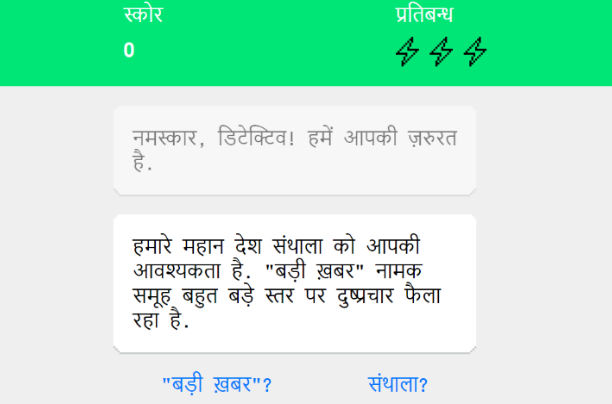
\includegraphics[height=.3\linewidth]{media/image3a.jpeg}
    
\includegraphics[height=.3\linewidth]{media/image3b.jpg}
    \caption{The first two messages after starting the game. \\The top message reads “Hello Detective! We need you.” The bottom message reads “Our great country Santhala needs you. A group called ‘Big News' is spreading propaganda on a very large scale” (left). \\In-game screenshot from the first level. The top message reads “Well done! Find the profile of a person who is a fake doctor.” The bottom message reads “Dr. Saurav Agrawal” (right).}
    \label{fig:figure3}
  \end{fullwidth}
\end{figure*}



At the end of each level, players are given a summary of the techniques they have been inoculated against. Points and sanctions are also counted throughout; if players send a message that does not reflect use of the techniques learned, they are penalized. Conversely, exposing propaganda as an undercover detective increases points. In all scenarios, players also see \mbox{WhatsApp} group members' reactions to the misinformation. Overall, the game aims to demonstrate how fabricated content can evoke not only belief in misinformation but also create an atmosphere of fear, polarization, and elicit violent offline behavior.

The study was thus designed to test the efficacy of \emph{Join this Group}, measured by three forms of assessment. We therefore hypothesized that:

\textbf{H}\textsubscript{\textbf{1}} Treatment group participants find manipulative \mbox{WhatsApp} messages significantly less reliable post-gameplay compared to the control group.

\textbf{H}\textsubscript{\textbf{2}} Treatment group participants are significantly more confident at assessing the reliability of manipulative \mbox{WhatsApp} messages compared to the control group.

\textbf{H}\textsubscript{\textbf{3}} Treatment group participants are significantly less likely to want to forward manipulative \mbox{WhatsApp} messages to others compared to the control group.

\section{Sample }

After providing informed consent, we collected \emph{n} = 1283 observations, of which, \emph{n} = 757 were complete responses. Participants did not always complete the full survey; we saw some drop-off after the intervention as many participants did not complete the post-test. To understand if the data was missing at random (MAR), we ran further analyses using the pre-test scores, condition allocation and \mbox{WhatsApp} usage data to assess missingness (see the supplementary materials for full details). We were not able to study the demographic predictors of the incomplete data because this was collected at the end of the study. The analysis finds that the data was not missing at random and that a higher baseline confidence in assessing the reliability of manipulative items decreased the odds of missingness (\emph{OR} = 0.030, [95\%\emph{CI}; 0.002,0.431]) and being assigned to the treatment group increased the odds of missingness (\emph{OR} = 2.171, [95\%\emph{CI}; 1.589, 2.967]). Please see Table S1 for full results.


\begin{table}[h!]

  \begin{fullwidth}
    \caption{A summary of the game from the player's perspective at each of the four levels. }
    \label{tab:table1}


    \begin{tabularx}{\linewidth}{@{}l  l  >{\RaggedRight\arraybackslash}X@{}}

      \emph{Level} & \emph{Manipulation Technique} & \emph{Description}                                                                                                                                                                                                                                                                                                                                                                                        \\
      1            & Fake Expert                   & As undercover detectives, players join a \mbox{WhatsApp} group called “Breaking News” in the town of “Santhala.” They share a fake message but are kicked out of the group, upon which they are encouraged to use a fake expert to gain credibility and witness how this impersonation can garner belief.                                                                                                 \\
      2            & Emotional Language            & Players are told that certain users in the group “Big News” are picking fights. As an undercover detective, they are tasked with spreading content to contribute to the chaos. The game then prompts players to share a fear or anger inducing message. This level shows players how, especially when paired with an image, emotional language can manipulate opinions and exacerbate chaos in the group. \\
      3            & Polarization                  & At this stage, Santhala is facing an election that the group “Breaking News” is attempting to manipulate. Players are told they must go undercover in one of the political candidate groups to spread polarizing information (e.g., damaging information about the opposition). The game shows how this cycle causes wider rifts between supporters.                                                      \\
      4            & Escalation                    & Continuing in context, the opposition group reports the polarizing fake news shared earlier to the media. The player is shown how members of the group try to identify the ‘mole' which escalates into an offline attack on the suspected individual. Although \mbox{WhatsApp} now bans this political group, players are shown how they simply create another one with new phone numbers.                \\
    \end{tabularx}

  \end{fullwidth}

\end{table}

During the data quality check, we further observed data in which participants just provided the same scale point consistently throughout the pre-test, post-test, or both (e.g., “4”). We therefore removed any responses which had repeated answer patterns\footnote{Analysis including the excluded 32 responses was also run and these did not affect the results.} throughout the entire section (pre-test or post-test), resulting in a final sample size of \emph{n} = 725. Of the final sample, 55\% identified as female, 40\% as male and 5\% as other. 49\% reported being 18-24 years old. 42\% reported having obtained at least a bachelor's degree. The sample was also heavily left leaning, (\emph{M} = 2.14, \emph{SD} = 0.78). Finally, 65\% of participants came from the state of Madhya Pradesh (17\% from Rajasthan, 6\% from Chhattisgarh, 5\% from Uttar Pradesh, 4\% from Jharkhand, 3\% from Bihar). See Table S2 for a full breakdown of the sample.

\section{Results }

All data cleaning and analysis was conducted using RStudio, scripts are available via the Open Science Framework: \url{https://osf.io/abjrg}. For the main analyses, the following packages were used: stats (for ANCOVA), TOSTER (for tests of statistical equivalence) and BayesFactor (for Bayesian t-tests).

We conducted a one-way ANCOVA to test \textbf{H}\textsubscript{\textbf{1}},\textbf{ }examining whether post-test reliability scores of manipulative items were significantly different between conditions, controlling for pre-test scores. We found no significant difference in reliability assessments between treatment and condition groups: \emph{F}(1,722) = 0.00, \emph{p} = 0.97. This relationship held for the subcategories of the fake items; fake expert: \emph{F}(1,722) = 0.21, \emph{p }= 0.65; emotion: \emph{F}(1,722) = 0.21, \emph{p }= 0.65; polarization: \emph{F}(1,722) = 0.35, \emph{p }=0.55; and escalation: \emph{F}(1,722) = 0.03, \emph{p} = 0.85. To test whether the non-significant results imply null effects or equivalence to zero \parencite{Lakens2018}, we conducted an equivalence test using two one-sided tests (TOST) on the post-gameplay outcomes (TOSTs).\footnote{The smallest effect size of interest (SESOI) was set to d = ±0.25 based on the smallest observed effect size found in published experiments that use gamified inoculation interventions \parencite{Roozenbeek2019}.} We could not confirm statistical equivalence to zero for the average reliability score \emph{t}(721.68) = -1.44, \emph{p} = 0.07. However, a Bayesian paired samples \emph{t}-test for the averaged reliability score of misinformation items gives a Bayes factor of \emph{BF}\textsubscript{\emph{10 }}= 0.25 (error \% = 0.00)\textbf{,} indicating support for the null hypothesis of \textbf{H}\textsubscript{\textbf{1}} \parencite{Dienes2014}.

To test \textbf{H}\textsubscript{\textbf{2}}\textbf{, }we followed the same analysis: we conducted a one-way ANCOVA on the average post-test confidence in reliability judgment scores, controlling for the baseline. We find no significant difference between groups: \emph{F}(1,722) = 1.79,\emph{ p} = 0.18 or for the subcategories; fake expert: \emph{F}(1, 722) = 1.56, \emph{p} = 0.21; emotion: \emph{F}(1,722) = 1.05, \emph{p} = 0.31; polarization: \emph{F}(1,722) = 1.18, \emph{p} = 0.28; escalation: \emph{F}(1,722) = 1.17, \emph{p} = 0.28. A TOST equivalence test confirmed equivalence to zero for the average post-test confidence scores (in assessing the reliability of misinformation items), \emph{t}(721.43) = -2.34, \emph{p }= 0.01. A Bayesian \emph{t}-test provided strong evidence for the null hypothesis of \textbf{H}\textsubscript{\textbf{2}}, with a Bayes factor of \emph{BF}\textsubscript{\emph{10 }}= 0.04 (error \% = 0.00).\textbf{ }

To test \textbf{H}\textsubscript{\textbf{3}}, or whether there was a difference in post-test scores of intended willingness to share misinformation, another one-way ANCOVA was conducted on the average post-test scores, controlling for the baseline. Results were non-significant \emph{F}(1,722) = 1.46, \emph{p }= 0.23 including on the subcategories; fake expert: \emph{F}(1,722) = 1.94, \emph{p }= 0.16; emotion: \emph{F}(1,722) = 0.29, \emph{p} = 0.59; polarization: \emph{F}(1,722) = 2.75, \emph{p} = 0.10; and escalation: \emph{F}(1,722) = 2.77, \emph{p} = 0.10. A TOST analysis on the post-test likelihood to share misinformation items scores could not confirm statistical equivalence to zero \emph{t}(719.73) = -0.64\emph{, p} = 0.26. However, a Bayesian \emph{t}-test suggested strong support for the null hypothesis of \textbf{H}\textsubscript{\textbf{3}}\textbf{ }with\textbf{ }a\textbf{ }Bayes factor of \emph{BF}\textsubscript{\emph{10}} = 0.07 (error \% = 0.00). See Table S6 for Bayesian \emph{t}-tests. Figure \ref{fig:figure4} shows the distribution of mean scores (reliability, confidence and sharing) for all misinformation items. Similarly, Figure \ref{fig:figure5} displays the distribution of mean reliability scores broken down by technique.

Though not hypothesized, to test whether the intervention increased skepticism towards factual messages, we also conducted a one-way ANCOVA to test for significant differences in post-gameplay scores for real news items, controlling for baseline scores. Specifically, ratings of reliability: \emph{F}(1,722) = 0.09, \emph{p} = 0.76; confidence in judgments: \emph{F}(1,722) = 1.10, \emph{p} = 0.30; and likelihood to share: \emph{F}(1,722) = 1.39, \emph{p }= 0.24 were not significantly different across treatment and control groups. Similarly, we tested whether the intervention improved participants assessments of the two genuine screenshots capturing fake news sharing on \mbox{WhatsApp}. Using one-way ANCOVAs we found no significant differences in ratings of reliability: \emph{F}(1, 712) = 0.99, \emph{p} = 0.32; confidence: \emph{F}(1, 711) = 1.68 , \emph{p }= 0.20; or likelihood to share: \emph{F}(1,702) = 0.12 , \emph{p }= 0.73.


\begin{figure*}[t]

  \begin{fullwidth}
    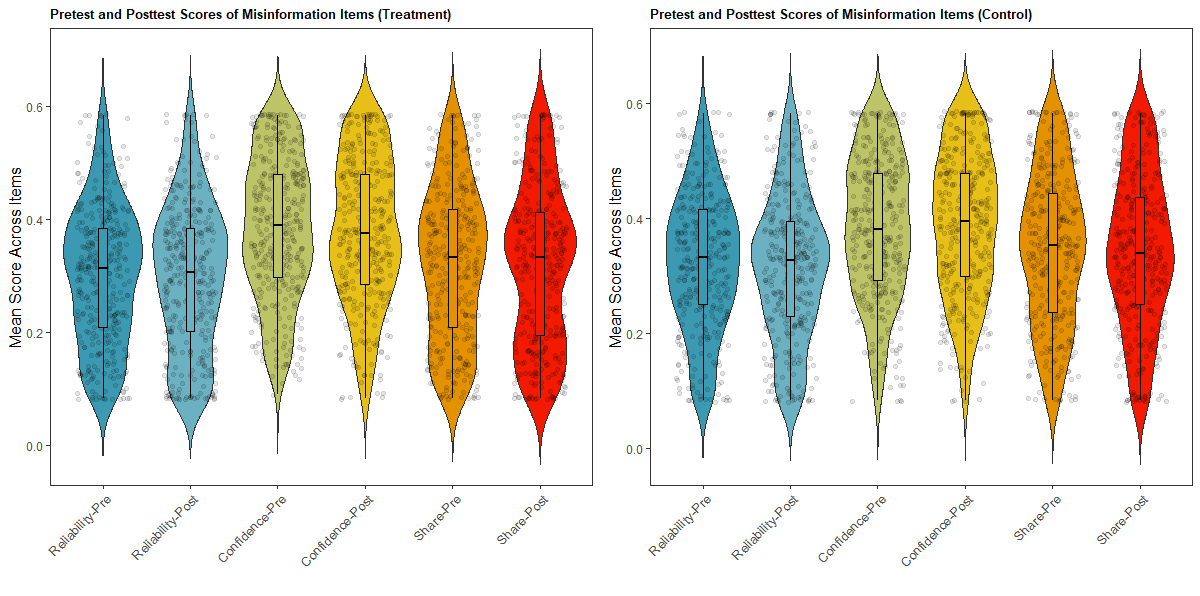
\includegraphics[width=\linewidth]{media/image4.jpeg}
    \caption{Distribution of pre-test and post-test mean scores in the treatment and control groups, for the reliability, confidence, and sharing scores of misinformation items across all manipulation techniques.}
    \label{fig:figure4}
  \end{fullwidth}


\end{figure*}




\begin{figure*}[t]

  \begin{fullwidth}
    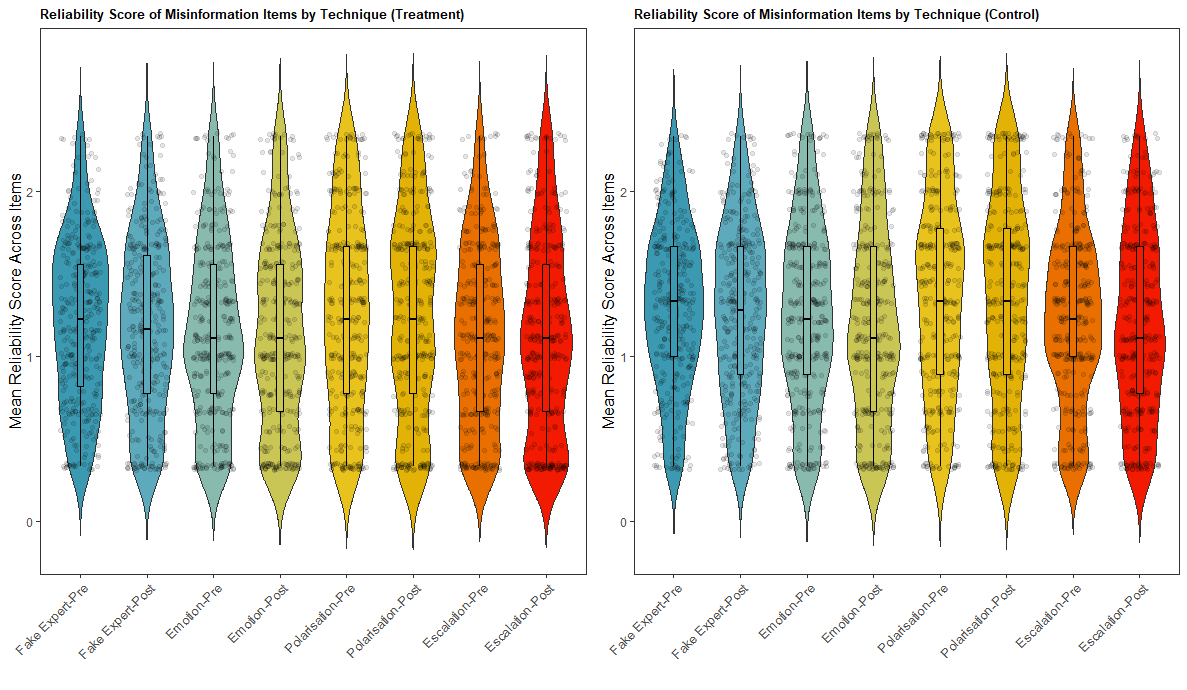
\includegraphics[width=\linewidth]{media/image3.jpeg}
    \caption{Distribution of mean reliability scores of misinformation items by manipulation technique. }
    \label{fig:figure5}
  \end{fullwidth}


\end{figure*}





We ran linear regressions to check for covariate effects on the differences in pre-post measures of reliability, confidence, and sharing. We only find that higher frequency of checking the news significantly predicts a larger difference between pre and post confidence scores of misinformation items (\emph{p = }0.03). See Tables S33-S35 for the full results.


\section{Discussion}

Through this study we demonstrate that there was no significant effect of playing \emph{Join this Group }on the veracity evaluations of both real and misinformation items in our sample of North Indians. This is in contrast with previous results that have found promising results using gamified inoculation in Western populations ( including versions translated to German, Greek, French, Polish, and Swedish \parencite{Basol2021, Roozenbeek2020}. Direct replications of the \emph{Bad News} game online have also shown positive effects on urban populations in India \parencite{Iyengar2022} and importantly, randomized trial data\footnote{ This publication of this data is forthcoming. Once published, it can be made available upon request.} from a representative sample of the UK population using the English version of \emph{Join this Group} found that the game significantly improved people's ability to detect fake news, how confident they were in their own judgments, and reduced their overall willingness to share misinformation with others \parencite{Basol2022}.

\begin{figure*}[t]

  \begin{fullwidth}
    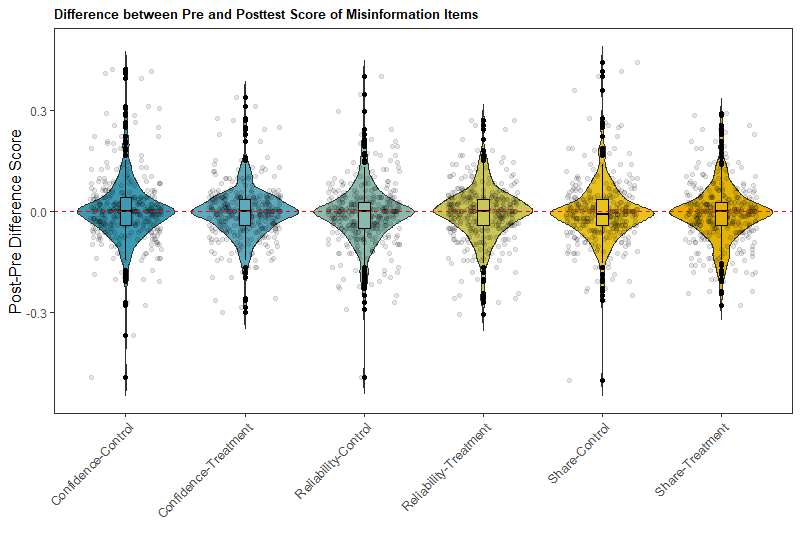
\includegraphics[width=\linewidth]{media/image6.jpeg}
    \caption{Distribution of post-pre differences between control and treatment groups. Red line drawn at y = 0.}
    \label{fig:figure6}
  \end{fullwidth}


\end{figure*}

There could be a myriad of explanations for the discrepant results observed. therefore, we categorize explanations into two broad categories: (1) cross-cultural (Indian sample, translated to Hindi) and (2) perspective shift (the player assumed the role of detective).

Firstly, we discuss possible cross-cultural explanations for our observed findings. While inoculation interventions demonstrate a clear potential to be effective \parencite{Traberg2022}, it is not surprising that the process of applying an intervention to understudied, non-WEIRD cultures \parencite{Henrich2010, Rad2018} might require an iterative process. Indeed, previous interventions aiming to reduce belief in and sharing of misinformation in India have faced similar difficulty. \mbox{WhatsApp}'s media literacy campaigns and adverts have been criticized for a lack of alignment with local contexts \parencite{Medeiros2021}. In-person or online digital literacy interventions have either demonstrated no reduced belief in misinformation \parencite{Badrinathan2021} or an effect size limited to a highly educated subset \parencite{Guess2020}. Here, we tested the efficacy of an inoculation intervention, \emph{Join this group, }that was modified for context through partnership with a local non-profit. The intervention aimed to teach participants fundamental techniques commonly used in the presentation of misinformation through an inoculation intervention. We expected that our local adaptation and use of inoculation would improve individual veracity discernment of manipulative news items. Yet, we do not find this in our study.

We hypothesize that the cultural context, local values, and social preferences may have played a role. In particular, the process of successful inoculation in the Indian population may be different. Threat has long been conceptualized a key and necessary component for inoculation to take place \parencite{McGuire1964} with most recent scholars agreeing that a threshold level of threat is required for inoculation to be conferred \parencite{Compton2021} as it serves the function of highlighting one's vulnerability which in turn, motivates the build-up of resistance. While there is no quantitatively defined level of minimum threat discussed in inoculation theory, studies assessing inoculation have traditionally measured threat as an apprehension \parencite{Ivanov2022, Wood2007} and more recently in a motivational form \parencite{Banas2017}. Unfortunately, we did not include measures of apprehensive or motivational threat in our study. Moreover, given the paucity of literature around non-WEIRD samples in psychology in general, it is difficult to make claims about the efficacy of inoculation without an explicit measurement of threat. Future research should consider incorporating this, informed by cultural variation in emotional experience and motivations \parencite{Kwan2016, Lim2004, Matsumoto2008, Mesquita2003}.

The cross-cultural adaptation also required numerous language and context changes. \parencite{Roozenbeek2020}. For example, the chosen fictional country of “Santhala” may have carried pre-conceived notions for some given its close resemblance to the Santhal tribe \parencite{EncyclopaediaBritannica2012}. All 12 manipulative \mbox{WhatsApp} prompts were translated from English to Hindi, which may have resulted in a loss of meaning and validity of measurement (see Figure S9 for an example). In addition, based on 2011 national census data, we estimate that our sample is 74\% rural \parencite{India2016}, a figure calculated based on the sample's distribution across states (see Table S39). \textcite{Shahid2022} find that rural samples had a lower ability to detect misinformation compared to their urban counterparts, suggesting that interventions on rural samples may require additional challenges.

Moreover, rural areas are estimated to have a digital literacy rate of 25\% compared to 61\% in urban areas \parencite{Mothkoor2021}, suggesting that our sample has low digital literacy overall. Classifying a household as digitally literate only requires one person, aged above 5 years, to be able to operate a computer and use the internet. As such, it is likely that our game-based intervention was conducted on participants with minimal experience with operating digital devices. This is compounded by the fact that the majority of our sample was female (55\%), who typically have lower digital literacy in this area \parencite{Rowntree2020}. This could have hindered the intervention's efficacy. Furthermore, data quality was poor: only 26\% of individuals who played the inoculation game put in the password correctly. Further analysis, however, demonstrated that this did not make a difference to our results (please see Tables S36-38).

Secondly, the game departed from previous game-based inoculation experiments in that it changed the player's perspective from troll to detective. Although this change preserved the critical element of ‘active' inoculation that has been effective previously \parencite{Pfau2005,Roozenbeek2019}, it is possible that the role of being not only a detective, but also being undercover, added further layers of complexity that minimized goal salience and clarity for participants, thus reducing its effectiveness. Practitioners may also consider running naturalistic studies in developing countries by conducting interventions broadcasted on \mbox{WhatsApp} through local organizations' subscription lists for increased data availability \parencite{Bowles2020}, or even by artificially constructing a social network in the lab \parencite{Pogorelskiy2017}.

\begin{originalPurpose}
  This paper aims to address the paucity of empirical research investigating misinformation interventions in developing countries. One important difference in the circulation of misinformation in developing countries is its spread through private, encrypted networks such as \mbox{WhatsApp}, which poses different challenges than (the circulation of) misinformation on open networks such as Twitter and Facebook. As such, this paper features a study testing the efficacy of an “inoculation” game in India. We hypothesized that previously reported effects of this inoculation game would be replicated by reducing the reported reliability and sharing intent of misinformation while increasing people's confidence in their own assessments.
\end{originalPurpose}

Our study may be taken as a lesson in conducting interventions in underexplored populations. In particular, the typical data quality, representativeness, and methodological best practices for running such online experiments in India, and non-WEIRD countries in general, is poorly understood and can impede the experimental process. \textcite{Campbell-Smith2019} notes, “having digital connectivity does not mean people are digitally equipped to use online surveys. They have issues in reading and writing, but not in talking.” Although we partnered with a local NGO in India, one must also account for gaps in the implementation of scientific experimental designs in the field, particularly by non-academic partners as it can increase the possibility of unobserved extraneous variables. Additionally, we observed non-random missingness in the data. We find that being assigned to the treatment group increases the odds of an incomplete or missing response, which may have introduced a bias in the results. However, as we found null results no further correction analysis was conducted. Future replications, particularly that find significant results, should pay attention to any differential attrition.

Future studies may also benefit from stronger local relationships \parencite{Sircar2019} as well as a greater accountability of the diversity within countries, such as India, that have notable heterogeneity beyond age, gender, and education level \parencite{Deshmukh2019}. For example, the question on political ideology in this study was more accurately asking people how “free” their ideology is rather than measuring their political ideology on a left-right scale (measure detailed in the supplement). Although India has been historically classified as clientelist and thus there is no established scale to capture political ideology, some evidence suggests voting behavior among certain groups is not clientelist \parencite{Chibber2018}. Future research will need to account for this in the design of surveys. In the context of misinformation, educational interventions have shown differing efficacy depending on political party support \parencite{Badrinathan2021} while polarizing content on the basis of religion and caste is often featured in misinformation circulated in India \parencite{Al-Zaman2021, Arun2019, Campbell-Smith2019}. For digital interventions, Indian samples may also vary in levels of digital literacy by caste and consumption levels \parencite{Mothkoor2021}. Therefore, additional measures, such as whether someone is part of a scheduled group (caste or tribe), religion, income level, and political party affiliation can facilitate a richer understanding of the intervention efficacy in subgroups due to heterogeneity in local factors. To isolate the effect of culture, experiments may also aspire to reach a more digitally literate population within non-WEIRD cultures, given that middle class, urban population in non-WEIRD countries are more likely to resemble the typically studied WEIRD population \parencite{Ghai2021}.

\section{Conclusion}

This study was motivated by scarcity of studies examining non-WEIRD populations in general \parencite{Henrich2010}, and by the lack of research testing the effectiveness of misinformation interventions in democracies such as India \parencite{Badrinathan2021}, that are being threatened by the prevalence of misinformation. We find null results of a game-based inoculation intervention, \emph{Join this Group, }on ratings of reliability, reported intent to share, and confidence in judgments of misinformation messages. Previous similar game-based inoculation interventions have been demonstrably successful \parencite{Basol2020, Roozenbeek2020, Roozenbeek2018, Roozenbeek2019, Roozenbeek2020}. We would thus conclude that the results reported here are more likely to reflect an interplay of cultural and experimental design factors. Taken together, we interpret these findings as a call for further adaptation and testing of inoculation interventions on non-WEIRD populations. Modifications may include measuring conceptual mediators such as motivational threat to elucidate and hypothesize potential differences in cross-cultural mechanisms, partnering with local researchers and universities, measuring digital literacy, as well as assessing of behavioral outcomes such as news sharing online.

\section{Acknowledgments}

We would like to thank our partners Digital Empowerment Foundation in India for implementing the survey and \mbox{WhatsApp}/Meta for funding.

\section{Funding}

This research was funded by \mbox{WhatsApp} through their \href{https://web.archive.org/web/20221118184849/https://www.whatsapp.com/research/awards/}{Research Awards for Social Science and Misinformation program.}

\newpage
\printbibliography
\appendix

\setcounter{figure}{0}

\setcounter{table}{0}
\captionsetup{
  labelformat=supplement
}
\onecolumn
\section{Supplemental Materials}

\subsection{Missing Data}
A total of \emph{n} = 1283 consenting individuals began the survey of which \emph{n} = 757 were complete and valid responses used in the analysis. As sample demographics were only collected after the post-test measures, it is not possible to understand the differences in individual characteristics across missing and complete responses. However, after filtering out for the those answered at least one question in the pre-test (\emph{n} = 1038), Little's MCAR test (run in R using the \emph{misty }package) for all three dependent variables (reliability, confidence and sharing) suggested that the data were not missing completely at random, χ\textsuperscript{2} (5) = 70.59, \emph{p }< 0.001. Thus, we ran a standard logistic regression (using the \emph{glm }function from the \emph{stats} package in R) to investigate patterns of missing data as a function of pre-test responses. This was done by creating a dummy variable where 1 = missing observation and 0 = complete responses. For the manipulative items, higher pre-test confidence scores slightly reduced the odds of missingness (\emph{OR} = 0.030, [95\%\emph{CI}; 0.002,0.431]) and being assigned the treatment group increased the odds of missingness (\emph{OR} = 2.171, [95\%\emph{CI}; 1.589, 2.967]). This implies that a higher baseline confidence in assessing the reliability of manipulative items decreases the likelihood of missingness while being assigned to the treatment group increases the likelihood of missingness. All other pre-test measures did not affect the odds of dropout. We were not able to assess whether the missing data was due to demographic factors as these were collected at the end of the study.



\begin{table}[h!]

  \caption{Logistic Regression Predicting Missingness (where Missing data = 1, Complete data = 0) }
  \label{tab:tableS1}


  \begin{tabularx}{\linewidth}{@{} X  l  l@{}}

    \toprule                               & Odds Ratio                   & Confidence Intervals      \\
    \midrule
    (Intercept)                            & 0.408                        & \emph{CI} [0.142, 1.172]  \\
    Reliability Pre-test (Fake Items)      & 0.836                        & \emph{CI} [0.082, 8.490]  \\
    Confidence Pre-test (Fake Items)       & 0.030 **                     & \emph{CI} [0.002, 0.431]  \\
    Sharing Pre-test (Fake Items)          & 4.965                        & \emph{CI} [0.509, 48.440] \\
    \mbox{WhatsApp} Usage                  & 1.032                        & \emph{CI} [0.848, 1.256]  \\
    Reliability Pre-test (Real Items)      & 1.100                        & \emph{CI} [0.849, 1.425]  \\
    Confidence Pre-test (Real Items)       & 0.811                        & \emph{CI} [0.626, 1.053]  \\
    Sharing Pre-test (Real Items)          & 1.034                        & \emph{CI} [0.806, 1.327]  \\
    Reliability Pre-test (Real Fake Items) & 1.067                        & \emph{CI} [0.800, 1.424]  \\
    Confidence Pre-test (Real Fake Items)  & 0.874                        & \emph{CI} [0.660, 1.157]  \\
    Sharing Pre-test (Real Fake Items)     & 1.307                        & \emph{CI} [0.942, 1.813]  \\
    Condition (Treatment)                  & 2.171 ***                    & \emph{CI} [1.589, 2.967]  \\
    \midrule
    N                                      & \multicolumn{2}{c}{899}                                  \\
    AIC                                    & \multicolumn{2}{c}{1057.126}                             \\
    BIC                                    & \multicolumn{2}{c}{1114.742}                             \\
    Pseudo R2                              & \multicolumn{2}{c}{0.083}                                \\
    \bottomrule
  \end{tabularx}
  *** p < 0.001; ** p < 0.01; * p < 0.05.


\end{table}



\clearpage
\subsection{ Political Ideology Measurements. }

Although we employed a measure from the British Social Attitudes survey, we employed a measure to assess the self-reported identification along the left to right spectrum: \\
नीचे दिए गए स्लाइडर पर, कृपया इंगित करें कि आप अपने आप को राजनीति के किस विचारधारा में देखते हैं.\\

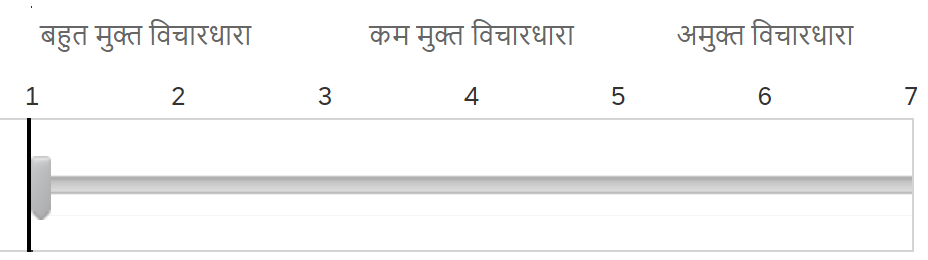
\includegraphics[width=\linewidth]{media/supplement/images-2.jpeg}
\emph{On the slider below, please indicate your political ideology.}\\
\emph{[Far left of slider; closer to 1] Very free ideology}\\
\emph{[Middle of slider; closer to 4] Less free ideology}\\
\emph{[Far right of slider; closer to 7] Not free ideology }
















\begin{table}
  \caption{Sample Composition}
  \label{tab:tableS2}

  \tiny
  \begin{tabularx}{\linewidth}{@{} X  r  r r@{}}

    \toprule
    \emph{Variable}                         & \emph{n} & \emph{Percentage} & \emph{Cumulative Percentage} \\
    \midrule

    \textbf{Gender}                         &          &                   &                              \\
    Male                                    & 293      & 40\%              & 40\%                         \\
    Female                                  & 397      & 55\%              & 95\%                         \\
    Other                                   & 35       & 5\%               & 100\%                        \\
    \textbf{Age}                            &          &                   &                              \\
    18-24                                   & 356      & 49\%              & 49\%                         \\
    25-34                                   & 286      & 39\%              & 89\%                         \\
    35-44                                   & 64       & 9\%               & 97\%                         \\
    45-54                                   & 16       & 2\%               & 100\%                        \\
    55 and over                             & 3        & 0\%               & 100\%                        \\
    \textbf{Political Leaning}              &          &                   &                              \\
    1 Very left-wing                        & 139      & 19\%              & 19\%                         \\
    2                                       & 385      & 53\%              & 72\%                         \\
    3                                       & 165      & 23\%              & 95\%                         \\
    4                                       & 34       & 5\%               & 100\%                        \\
    5 Very right-wing                       & 2        & 0\%               & 100\%                        \\
    \textbf{Education}                      &          &                   &                              \\
    Class 12                                & 159      & 22\%              & 22\%                         \\
    Elementary                              & 16       & 2\%               & 24\%                         \\
    Graduate                                & 306      & 42\%              & 66\%                         \\
    Post Grad                               & 172      & 24\%              & 90\%                         \\
    Up to Tenth                             & 72       & 10\%              & 100\%                        \\
    \textbf{State}                          &          &                   &                              \\
    Bihar                                   & 19       & 3\%               & 3\%                          \\
    Chhattisgarh                            & 42       & 6\%               & 8\%                          \\
    Delhi                                   & 3        & 0\%               & 9\%                          \\
    Haryana                                 & 5        & 1\%               & 10\%                         \\
    Jharkhand                               & 26       & 4\%               & 13\%                         \\
    Madhya Pradesh                          & 471      & 65\%              & 78\%                         \\
    Rajasthan                               & 120      & 17\%              & 95\%                         \\
    Unknown                                 & 6        & 1\%               & 95\%                         \\
    Uttar Pradesh                           & 33       & 5\%               & 100\%                        \\
    \textbf{Frequency of Checking the News} &          &                   &                              \\
    1 Never                                 & 5        & 1\%               & 1\%                          \\
    2 Occasionally                          & 90       & 12\%              & 13\%                         \\
    3 Somewhat                              & 166      & 23\%              & 36\%                         \\
    4 Often                                 & 295      & 41\%              & 77\%                         \\
    5 All the time                          & 169      & 23\%              & 100\%                        \\
  \end{tabularx}


\end{table}

\addtocounter{table}{-1}

\begin{table}

  \caption{Table S\ref{tab:tableS2} continued}

  \begin{tabularx}{\linewidth}{@{} X r r r @{}}
    \textbf{Use of social media }   &     &      &       \\
    1 Never                         & 28  & 4\%  & 4\%   \\
    2 Occasionally                  & 129 & 18\% & 22\%  \\
    3 Somewhat                      & 167 & 23\% & 45\%  \\
    4 Often                         & 212 & 29\% & 74\%  \\
    5 All the time                  & 189 & 26\% & 100\% \\
    \textbf{Use of \mbox{WhatsApp}} &     &      &       \\
    1 Never                         & 4   & 1\%  & 1\%   \\
    2 Occasionally                  & 22  & 3\%  & 4\%   \\
    3 Once a week                   & 26  & 4\%  & 7\%   \\
    4 Daily                         & 90  & 12\% & 20\%  \\
    5 More than once a day          & 520 & 72\% & 91\%  \\
    NA                              & 63  & 9\%  & 100\% \\
    \textbf{Interest in Politics}   &     &      &       \\
    1 Not interested at all         & 50  & 7\%  & 7\%   \\
    2                               & 84  & 12\% & 18\%  \\
    3 Slightly interested           & 289 & 40\% & 58\%  \\
    4                               & 189 & 26\% & 84\%  \\
    5 Very interested               & 113 & 16\% & 100\% \\
    \bottomrule
  \end{tabularx}
\end{table}


\begin{table}

  \caption{ANCOVA on Post-Treatment scores of reliability assessments (of manipulative items) }
  \label{tab:tableS3}


  \begin{tabularx}{\linewidth}{@{}  l  S  S  S  S  S  S  c  @{}}
    \toprule
    {Predictor} & {SumofSquares} & {\emph{df}} & {MeanSquare} & {\emph{F}} & {\emph{p}}       & {\textsubscript{partial }η\textsuperscript{2}} & \begin{tabular}{@{}c@{}}\textsubscript{partial }η\textsuperscript{2 }\\ 90\%\emph{CI}\\ {[}LL, UL{]} \end{tabular} \\
    \midrule


    (Intercept) & 0.25           & 1           & 0.25         & 36.90      & \emph{p} < 0.001 &                                                &                                                                                                                    \\
    F\_Rel\_Pre & 6.76           & 1           & 6.76         & 1000.84    & \emph{p} < 0.001 & .58                                            & [.55, .61]                                                                                                         \\
    Condition   & 0.00           & 1           & 0.00         & 0.00       & .969             & .00                                            & [.00, 1.00]                                                                                                        \\
    Error       & 4.88           & 722         & 0.01         &            &                  &                                                &                                                                                                                    \\
    \bottomrule
  \end{tabularx}


  \emph{Note.} LL and UL represent the lower-limit and upper-limit of the partial η\textsuperscript{2} confidence interval, respectively.
\end{table}

\textbf{}\begin{table}

  \caption{ANCOVA on Post-Treatment scores of confidence measure (of manipulative items) }
  \label{tab:tableS4}


  \begin{tabularx}{\linewidth}{@{}  l  S  S  S  S  S  S  c  @{}}
    \toprule
    {Predictor}  & {SumofSquares} & {\emph{df}} & {MeanSquare} & {\emph{F}} & {\emph{p}}       & {\textsubscript{partial }η\textsuperscript{2}} & \begin{tabular}{@{}c@{}}\textsubscript{partial }η\textsuperscript{2 }\\ 90\%\emph{CI}\\ {[}LL, UL{]} \end{tabular} \\


    \midrule
    (Intercept)  & 0.59           & 1           & 0.59         & 83.25      & \emph{p} < 0.001 &                                                &                                                                                                                    \\
    F\_Conf\_Pre & 6.45           & 1           & 6.45         & 908.30     & \emph{p} < 0.001 & .56                                            & [.52, .59]                                                                                                         \\
    Condition    & 0.01           & 1           & 0.01         & 1.79       & .181             & .00                                            & [.00, .01]                                                                                                         \\
    Error        & 5.13           & 722         & 0.01         &            &                  &                                                &                                                                                                                    \\
    \bottomrule
  \end{tabularx}


  \emph{Note.} LL and UL represent the lower-limit and upper-limit of the partial η\textsuperscript{2} confidence interval, respectively.
\end{table}



\begin{table}

  \caption{ANCOVA on Post-Treatment scores of sharing measure (of manipulative items)}
  \label{tab:tableS5}


  \begin{tabularx}{\linewidth}{@{}  l  S  S  S  S  S  S  c  @{}}
    \toprule
    {Predictor}   & {SumofSquares} & {\emph{df}} & {MeanSquare} & {\emph{F}} & {\emph{p}}       & {\textsubscript{partial }η\textsuperscript{2}} & \begin{tabular}{@{}c@{}}\textsubscript{partial }η\textsuperscript{2 }\\ 90\%\emph{CI}\\ {[}LL, UL{]} \end{tabular} \\


    \midrule
    (Intercept)   & 0.35           & 1           & 0.35         & 48.64      & \emph{p} < 0.001 &                                                &                                                                                                                    \\
    F\_Share\_Pre & 8.42           & 1           & 8.42         & 1155.91    & \emph{p} < 0.001 & .62                                            & [.58, .64]                                                                                                         \\
    Condition     & 0.01           & 1           & 0.01         & 1.46       & .227             & .00                                            & [.00, .01]                                                                                                         \\
    Error         & 5.26           & 722         & 0.01         &            &                  &                                                &                                                                                                                    \\
    \bottomrule
  \end{tabularx}


  \emph{Note.} LL and UL represent the lower-limit and upper-limit of the partial η\textsuperscript{2} confidence interval, respectively.
\end{table}







\begin{table}

  \caption{\textbf{ }\emph{Bayesian}\textbf{ }\emph{paired sample t-test on dependent variables }}
  \label{tab:tableS6}


  \begin{tabularx}{\linewidth}{@{} X  X  X  l  l@{}}


    \toprule
    \multicolumn{3}{c}{\textbf{Variable}}                                       & \textbf{Statistic } & \textbf{Error \%}                                                         \\
    \midrule
    \multicolumn{2}{@{} l @{}}{\emph{Reliability of Fake Messages }}            &                     &                                     &                                     \\
    Reliability-Post                                                            & Reliability-Pre     & BF\textsubscript{10, prior = 0.707} & 0.249 & 2.604E\textsuperscript{-08} \\
    \multicolumn{2}{@{} l @{}}{\emph{Confidence in judgement of Fake Messages}} &                     &                                     &                                     \\
    Confidence-Post                                                             & Confidence-Pre      & BF\textsubscript{10, prior = 0.707} & 0.043 & 1.612E\textsuperscript{-07} \\
    \multicolumn{2}{@{} l @{}}{\emph{Intent to share Fake Messages}}            &                     &                                     &                                     \\
    Share-Post                                                                  & Share-Pre           & BF\textsubscript{10, prior = 0.707} & 0.073 & 9.425E\textsuperscript{-08} \\
    \bottomrule
  \end{tabularx}


\end{table}


\begin{table}

  \caption{Reliability measure - Fixed-Effects ANCOVA on post-test fake expert manipulation items }
  \label{tab:tableS7}


  \begin{tabularx}{\linewidth}{@{}  l  S  S  S  S  S  S  c  @{}}
    \toprule
    {Predictor}  & {SumofSquares} & {\emph{df}} & {MeanSquare} & {\emph{F}} & {\emph{p}}       & {\textsubscript{partial }η\textsuperscript{2}} & \begin{tabular}{@{}c@{}}\textsubscript{partial }η\textsuperscript{2 }\\ 90\%\emph{CI}\\ {[}LL, UL{]} \end{tabular} \\
    \midrule

    (Intercept)  & 6.49           & 1           & 6.49         & 48.51      & \emph{p} < 0.001 &                                                &                                                                                                                    \\
    FE\_Rel\_Pre & 102.89         & 1           & 102.89       & 768.80     & \emph{p} < 0.001 & .52                                            & [.48, .55]                                                                                                         \\
    Condition    & 0.03           & 1           & 0.03         & 0.21       & .648             & .00                                            & [.00, .01]                                                                                                         \\
    Error        & 96.62          & 722         & 0.13         &            &                  &                                                &                                                                                                                    \\
    \bottomrule
  \end{tabularx}


  \emph{Note.} LL and UL represent the lower-limit and upper-limit of the partial η\textsuperscript{2} confidence interval, respectively.
\end{table}



\begin{table}

  \caption{Reliability Measure - ANCOVA on post-test score of emotional manipulation items }
  \label{tab:tableS8}


  \begin{tabularx}{\linewidth}{@{}  l  l  l  S  l  l  l  l @{}}
    \toprule
    {Predictor}  & {SumofSquares} & {\emph{df}} & {MeanSquare} & {\emph{F}} & {\emph{p}}       & {\textsubscript{partial }η\textsuperscript{2}} & \begin{tabular}{@{}c@{}}\textsubscript{partial }η\textsuperscript{2 }\\ 90\%\emph{CI}\\ {[}LL, UL{]} \end{tabular} \\
    \midrule

    (Intercept)  & 14.19          & 1           & 14.19        & 69.20      & \emph{p} < 0.001 &                                                &                                                                                                                    \\
    EM\_Rel\_Pre & 89.90          & 1           & 89.90        & 438.44     & \emph{p} < 0.001 & .38                                            & [.33, .42]                                                                                                         \\
    Condition    & 0.04           & 1           & 0.04         & 0.21       & .649             & .00                                            & [.00, .01]                                                                                                         \\
    Error        & 148.04         & 722         & 0.21         &            &                  &                                                &                                                                                                                    \\
    \bottomrule
  \end{tabularx}

  \emph{Note.} LL and UL represent the lower-limit and upper-limit of the partial η\textsuperscript{2} confidence interval, respectively.

\end{table}





\begin{table}

  \caption{Reliability Measure - ANCOVA on post-test score of polarisation manipulation items }
  \label{tab:tableS9}


  \begin{tabularx}{\linewidth}{@{}  l  S  S  S  S  S  S  c  @{}}
    \toprule
    {Predictor}  & {SumofSquares} & {\emph{df}} & {MeanSquare} & {\emph{F}} & {\emph{p}}       & {\textsubscript{partial }η\textsuperscript{2}} & \begin{tabular}{@{}c@{}}\textsubscript{partial }η\textsuperscript{2 }\\ 90\%\emph{CI}\\ {[}LL, UL{]} \end{tabular} \\
    \midrule

    (Intercept)  & 16.52          & 1           & 16.52        & 81.00      & \emph{p} < 0.001 &                                                &                                                                                                                    \\
    PL\_Rel\_Pre & 119.46         & 1           & 119.46       & 585.71     & \emph{p} < 0.001 & .45                                            & [.41, .49]                                                                                                         \\
    Condition    & 0.07           & 1           & 0.07         & 0.35       & .553             & .00                                            & [.00, .01]                                                                                                         \\
    Error        & 147.26         & 722         & 0.20         &            &                  &                                                &                                                                                                                    \\
    \bottomrule
  \end{tabularx}


  \emph{Note.} LL and UL represent the lower-limit and upper-limit of the partial η\textsuperscript{2} confidence interval, respectively.
\end{table}



\begin{table}

  \caption{ Reliability Measure - ANCOVA on post-test score of escalation manipulation items }
  \label{tab:tableS10}


  \begin{tabularx}{\linewidth}{@{}  l  S  S  S  S  S  S  c  @{}}
    \toprule
    {Predictor}  & {SumofSquares} & {\emph{df}} & {MeanSquare} & {\emph{F}} & {\emph{p}}       & {\textsubscript{partial }η\textsuperscript{2}} & \begin{tabular}{@{}c@{}}\textsubscript{partial }η\textsuperscript{2 }\\ 90\%\emph{CI}\\ {[}LL, UL{]} \end{tabular} \\
    \midrule

    (Intercept)  & 13.38          & 1           & 13.38        & 68.51      & \emph{p} < 0.001 &                                                &                                                                                                                    \\
    ES\_Rel\_Pre & 96.59          & 1           & 96.59        & 494.40     & \emph{p} < 0.001 & .41                                            & [.36, .45]                                                                                                         \\
    Condition    & 0.01           & 1           & 0.01         & 0.03       & .852             & .00                                            & [.00, .00]                                                                                                         \\
    Error        & 141.06         & 722         & 0.20         &            &                  &                                                &                                                                                                                    \\
    \bottomrule
  \end{tabularx}


  \emph{Note.} LL and UL represent the lower-limit and upper-limit of the partial η\textsuperscript{2} confidence interval, respectively.
\end{table}





\begin{table}

  \caption{\textbf{ }\emph{Reliability measure -- ANCOVA on post-test score of authentic fake news items }}
  \label{tab:tableS11}


  \begin{tabularx}{\linewidth}{@{}  l  S  S  S  S  S  S  c  @{}}
    \toprule
    {Predictor}  & {SumofSquares} & {\emph{df}} & {MeanSquare} & {\emph{F}} & {\emph{p}} & {\textsubscript{partial }η\textsuperscript{2}} & \begin{tabular}{@{}c@{}}\textsubscript{partial }η\textsuperscript{2 }\\ 90\%\emph{CI}\\ {[}LL, UL{]} \end{tabular} \\
    \midrule

    (Intercept)  & 63.45          & 1           & 63.45        & 116.01     & .000       &                                                &                                                                                                                    \\
    RF\_Rel\_Pre & 198.77         & 1           & 198.77       & 363.43     & .000       & .34                                            & [.29, .38]                                                                                                         \\
    Condition    & 0.54           & 1           & 0.54         & 0.99       & .319       & .00                                            & [.00, .01]                                                                                                         \\
    Error        & 389.40         & 712         & 0.55         &            &            &                                                &                                                                                                                    \\
    \bottomrule
  \end{tabularx}


  \emph{Note.} LL and UL represent the lower-limit and upper-limit of the partial η\textsuperscript{2} confidence interval, respectively.
\end{table}



\begin{table}

  \caption{ Reliability measure - ANCOVA on post-test score of real (non-manipulative) items }
  \label{tab:tableS12}


  \begin{tabularx}{\linewidth}{@{}  l  S  S  S  S  S  S  c  @{}}
    \toprule
    {Predictor} & {SumofSquares} & {\emph{df}} & {MeanSquare} & {\emph{F}} & {\emph{p}} & {\textsubscript{partial }η\textsuperscript{2}} & \begin{tabular}{@{}c@{}}\textsubscript{partial }η\textsuperscript{2 }\\ 90\%\emph{CI}\\ {[}LL, UL{]} \end{tabular} \\
    \midrule

    (Intercept) & 41.14          & 1           & 41.14        & 81.48      & .000       &                                                &                                                                                                                    \\
    R\_Rel\_Pre & 265.29         & 1           & 265.29       & 525.46     & .000       & .42                                            & [.38, .46]                                                                                                         \\
    Condition   & 0.05           & 1           & 0.05         & 0.09       & .763       & .00                                            & [.00, .00]                                                                                                         \\
    Error       & 364.52         & 722         & 0.50         &            &            &                                                &                                                                                                                    \\
    \bottomrule
  \end{tabularx}


  \emph{Note.} LL and UL represent the lower-limit and upper-limit of the partial η\textsuperscript{2} confidence interval, respectively.
\end{table}



\begin{table}

  \caption{ Confidence measure - ANCOVA on post-test score of fake expert manipulation items }
  \label{tab:tableS13}


  \begin{tabularx}{\linewidth}{@{}  l  S  S  S  S  S  S  c  @{}}
    \toprule
    {Predictor}   & {SumofSquares} & {\emph{df}} & {MeanSquare} & {\emph{F}} & {\emph{p}}       & {\textsubscript{partial }η\textsuperscript{2}} & \begin{tabular}{@{}c@{}}\textsubscript{partial }η\textsuperscript{2 }\\ 90\%\emph{CI}\\ {[}LL, UL{]} \end{tabular} \\
    \midrule

    (Intercept)   & 16.56          & 1           & 16.56        & 123.94     & \emph{p} < 0.001 &                                                &                                                                                                                    \\
    FE\_Conf\_Pre & 96.67          & 1           & 96.67        & 723.45     & \emph{p} < 0.001 & .50                                            & [.46, .54]                                                                                                         \\
    Condition     & 0.21           & 1           & 0.21         & 1.56       & .211             & .00                                            & [.00, .01]                                                                                                         \\
    Error         & 96.47          & 722         & 0.13         &            &                  &                                                &                                                                                                                    \\
    \bottomrule
  \end{tabularx}


  \emph{Note.} LL and UL represent the lower-limit and upper-limit of the partial η\textsuperscript{2} confidence interval, respectively.
\end{table}



\begin{table}

  \caption{Confidence measure -- ANCOVA on post-test score of emotional manipulation items }
  \label{tab:tableS14}


  \begin{tabularx}{\linewidth}{@{}  l  S  S  S  S  S  S  c  @{}}
    \toprule
    {Predictor}   & {SumofSquares} & {\emph{df}} & {MeanSquare} & {\emph{F}} & {\emph{p}}       & {\textsubscript{partial }η\textsuperscript{2}} & \begin{tabular}{@{}c@{}}\textsubscript{partial }η\textsuperscript{2 }\\ 90\%\emph{CI}\\ {[}LL, UL{]} \end{tabular} \\
    \midrule

    (Intercept)   & 19.49          & 1           & 19.49        & 103.28     & \emph{p} < 0.001 &                                                &                                                                                                                    \\
    EM\_Conf\_Pre & 90.92          & 1           & 90.92        & 481.79     & \emph{p} < 0.001 & .40                                            & [.36, .44]                                                                                                         \\
    Condition     & 0.20           & 1           & 0.20         & 1.05       & .306             & .00                                            & [.00, .01]                                                                                                         \\
    Error         & 136.25         & 722         & 0.19         &            &                  &                                                &                                                                                                                    \\
    \bottomrule
  \end{tabularx}


  \emph{Note.} LL and UL represent the lower-limit and upper-limit of the partial η\textsuperscript{2} confidence interval, respectively.
\end{table}





\begin{table}
  \caption{Confidence measure -- ANCOVA on post-test score of polarisation manipulation items}


  \begin{tabularx}{\linewidth}{@{}  l  S  S  S  S  S  S  c  @{}}
    \toprule
    {Predictor}   & {SumofSquares} & {\emph{df}} & {MeanSquare} & {\emph{F}} & {\emph{p}}       & {\textsubscript{partial }η\textsuperscript{2}} & \begin{tabular}{@{}c@{}}\textsubscript{partial }η\textsuperscript{2 }\\ 90\%\emph{CI}\\ {[}LL, UL{]} \end{tabular} \\
    \midrule

    (Intercept)   & 22.17          & 1           & 22.17        & 119.57     & \emph{p} < 0.001 &                                                &                                                                                                                    \\
    PL\_Conf\_Pre & 92.32          & 1           & 92.32        & 497.93     & \emph{p} < 0.001 & .41                                            & [.37, .45]                                                                                                         \\
    Condition     & 0.22           & 1           & 0.22         & 1.18       & .278             & .00                                            & [.00, .01]                                                                                                         \\
    Error         & 133.87         & 722         & 0.19         &            &                  &                                                &                                                                                                                    \\
    \bottomrule
  \end{tabularx}


  \emph{Note.} LL and UL represent the lower-limit and upper-limit of the partial η\textsuperscript{2} confidence interval, respectively.
\end{table}

















\begin{table}

  \caption{Confidence measure -- ANCOVA on post-test score of escalation manipulation items}

  \begin{tabularx}{\linewidth}{@{}  l  S  S  S  S  S  S  c  @{}}
    \toprule
    {Predictor}   & {SumofSquares} & {\emph{df}} & {MeanSquare} & {\emph{F}} & {\emph{p}}       & {\textsubscript{partial }η\textsuperscript{2}} & \begin{tabular}{@{}c@{}}\textsubscript{partial }η\textsuperscript{2 }\\ 90\%\emph{CI}\\ {[}LL, UL{]} \end{tabular} \\
    \midrule

    (Intercept)   & 24.97          & 1           & 24.97        & 135.70     & \emph{p} < 0.001 &                                                &                                                                                                                    \\
    ES\_Conf\_Pre & 90.68          & 1           & 90.68        & 492.84     & \emph{p} < 0.001 & .41                                            & [.36, .45]                                                                                                         \\
    Condition     & 0.21           & 1           & 0.21         & 1.17       & .280             & .00                                            & [.00, .01]                                                                                                         \\
    Error         & 132.84         & 722         & 0.18         &            &                  &                                                &                                                                                                                    \\
    \bottomrule
  \end{tabularx}


  \emph{Note.} LL and UL represent the lower-limit and upper-limit of the partial η\textsuperscript{2} confidence interval, respectively.
\end{table}





\begin{table}

  \caption{Confidence measure -- ANCOVA on post-test score of authentic fake news items}

  \begin{tabularx}{\linewidth}{@{}  l  S  S  S  S  S  S  c  @{}}
    \toprule
    {Predictor}   & {SumofSquares} & {\emph{df}} & {MeanSquare} & {\emph{F}} & {\emph{p}} & {\textsubscript{partial }η\textsuperscript{2}} & \begin{tabular}{@{}c@{}}\textsubscript{partial }η\textsuperscript{2 }\\ 90\%\emph{CI}\\ {[}LL, UL{]} \end{tabular} \\
    \midrule

    (Intercept)   & 72.95          & 1           & 72.95        & 143.40     & .000       &                                                &                                                                                                                    \\
    RF\_Conf\_Pre & 200.25         & 1           & 200.25       & 393.60     & .000       & .36                                            & [.31, .40]                                                                                                         \\
    Condition     & 0.86           & 1           & 0.86         & 1.68       & .195       & .00                                            & [.00, .01]                                                                                                         \\
    Error         & 361.73         & 711         & 0.51         &            &            &                                                &                                                                                                                    \\
    \bottomrule
  \end{tabularx}


  \emph{Note.} LL and UL represent the lower-limit and upper-limit of the partial η\textsuperscript{2} confidence interval, respectively.
\end{table}



\begin{table}

  \caption{Confidence measure -- ANCOVA on post-test score of real (non-manipulative) items}
  \label{tab:tableS18}


  \begin{tabularx}{\linewidth}{@{}  l  S  S  S  S  S  S  c  @{}}
    \toprule
    {Predictor}  & {SumofSquares} & {\emph{df}} & {MeanSquare} & {\emph{F}} & {\emph{p}} & {\textsubscript{partial }η\textsuperscript{2}} & \begin{tabular}{@{}c@{}}\textsubscript{partial }η\textsuperscript{2 }\\ 90\%\emph{CI}\\ {[}LL, UL{]} \end{tabular} \\
    \midrule

    (Intercept)  & 64.69          & 1           & 64.69        & 110.28     & .000       &                                                &                                                                                                                    \\
    R\_Conf\_Pre & 325.73         & 1           & 325.73       & 555.32     & .000       & .43                                            & [.39, .47]                                                                                                         \\
    Condition    & 0.65           & 1           & 0.65         & 1.10       & .295       & .00                                            & [.00, .01]                                                                                                         \\
    Error        & 423.49         & 722         & 0.59         &            &            &                                                &                                                                                                                    \\
    \bottomrule
  \end{tabularx}


  \emph{Note.} LL and UL represent the lower-limit and upper-limit of the partial η\textsuperscript{2} confidence interval, respectively.
\end{table}



\begin{table}

  \caption{ Sharing Measure -- ANCOVA on post-test score of fake expert manipulation items }
  \label{tab:tableS19}


  \begin{tabularx}{\linewidth}{@{}  l  S  S  S  S  S  S  c  @{}}
    \toprule
    {Predictor}    & {SumofSquares} & {\emph{df}} & {MeanSquare} & {\emph{F}} & {\emph{p}}       & {\textsubscript{partial }η\textsuperscript{2}} & \begin{tabular}{@{}c@{}}\textsubscript{partial }η\textsuperscript{2 }\\ 90\%\emph{CI}\\ {[}LL, UL{]} \end{tabular} \\
    \midrule

    (Intercept)    & 10.08          & 1           & 10.08        & 69.52      & \emph{p} < 0.001 &                                                &                                                                                                                    \\
    FE\_Share\_Pre & 125.70         & 1           & 125.70       & 867.08     & \emph{p} < 0.001 & .55                                            & [.51, .58]                                                                                                         \\
    Condition      & 0.28           & 1           & 0.28         & 1.94       & .164             & .00                                            & [.00, .01]                                                                                                         \\
    Error          & 104.67         & 722         & 0.14         &            &                  &                                                &                                                                                                                    \\
    \bottomrule
  \end{tabularx}


  \emph{Note.} LL and UL represent the lower-limit and upper-limit of the partial η\textsuperscript{2} confidence interval, respectively.
\end{table}



\begin{table}

  \caption{Sharing Measure -- ANCOVA on post-test score of emotional manipulation items }
  \label{tab:tableS20}


  \begin{tabularx}{\linewidth}{@{}  l  S  S  S  S  S  S  c  @{}}
    \toprule
    {Predictor}    & {SumofSquares} & {\emph{df}} & {MeanSquare} & {\emph{F}} & {\emph{p}}       & {\textsubscript{partial }η\textsuperscript{2}} & \begin{tabular}{@{}c@{}}\textsubscript{partial }η\textsuperscript{2 }\\ 90\%\emph{CI}\\ {[}LL, UL{]} \end{tabular} \\
    \midrule

    (Intercept)    & 13.68          & 1           & 13.68        & 67.67      & \emph{p} < 0.001 &                                                &                                                                                                                    \\
    EM\_Share\_Pre & 133.09         & 1           & 133.09       & 658.41     & \emph{p} < 0.001 & .48                                            & [.44, .51]                                                                                                         \\
    Condition      & 0.06           & 1           & 0.06         & 0.29       & .590             & .00                                            & [.00, .01]                                                                                                         \\
    Error          & 145.95         & 722         & 0.20         &            &                  &                                                &                                                                                                                    \\
    \bottomrule
  \end{tabularx}


  \emph{Note.} LL and UL represent the lower-limit and upper-limit of the partial η\textsuperscript{2} confidence interval, respectively.
\end{table}





\begin{table}

  \caption{Sharing Measure -- ANCOVA on post-test score of polarisation manipulation items }
  \label{tab:tableS21}


  \begin{tabularx}{\linewidth}{@{} l  S  S  S  S  S  S  c @{}}

    \toprule
    {Predictor}    & {SumofSquares} & {\emph{df}} & {MeanSquare} & {\emph{F}} & {\emph{p}}       & {\textsubscript{partial }η\textsuperscript{2}} & \begin{tabular}{@{}c@{}}\textsubscript{partial }η\textsuperscript{2 }\\ 90\%\emph{CI}\\ {[}LL, UL{]} \end{tabular} \\
    \midrule
    (Intercept)    & 17.68          & 1           & 17.68        & 82.23      & \emph{p} < 0.001 &                                                &                                                                                                                    \\
    PL\_Share\_Pre & 130.23         & 1           & 130.23       & 605.59     & \emph{p} < 0.001 & .46                                            & [.41, .49]                                                                                                         \\
    Condition      & 0.59           & 1           & 0.59         & 2.75       & .098             & .00                                            & [.00, .01]                                                                                                         \\
    Error          & 155.26         & 722         & 0.22         &            &                  &                                                &                                                                                                                    \\
    \bottomrule
  \end{tabularx}


  \emph{Note.} LL and UL represent the lower-limit and upper-limit of the partial η\textsuperscript{2} confidence interval, respectively.
\end{table}



\begin{table}

  \caption{Sharing Measure -- ANCOVA on post-test score of escalation manipulation items }
  \label{tab:tableS22}


  \begin{tabularx}{\linewidth}{@{} l  S  S  S  S  S  S  c @{}}

    \toprule
    {Predictor}    & {SumofSquares} & {\emph{df}} & {MeanSquare} & {\emph{F}} & {\emph{p}}       & {\textsubscript{partial }η\textsuperscript{2}} & \begin{tabular}{@{}c@{}}\textsubscript{partial }η\textsuperscript{2 }\\ 90\%\emph{CI}\\ {[}LL, UL{]} \end{tabular} \\
    \midrule
    (Intercept)    & 17.43          & 1           & 17.43        & 88.22      & \emph{p} < 0.001 &                                                &                                                                                                                    \\
    ES\_Share\_Pre & 130.11         & 1           & 130.11       & 658.64     & \emph{p} < 0.001 & .48                                            & [.44, .51]                                                                                                         \\
    Condition      & 0.55           & 1           & 0.55         & 2.77       & .097             & .00                                            & [.00, .01]                                                                                                         \\
    Error          & 142.63         & 722         & 0.20         &            &                  &                                                &                                                                                                                    \\
    \bottomrule
  \end{tabularx}


  \emph{Note.} LL and UL represent the lower-limit and upper-limit of the partial η\textsuperscript{2} confidence interval, respectively.
\end{table}





\begin{table}
  \caption{Sharing measure -- ANCOVA on post-test score of authentic fake news items}
  \label{tab:tableS23}


  \begin{tabularx}{\linewidth}{@{} l  S  S  S  S  S  S  c @{}}

    \toprule
    {Predictor}    & {SumofSquares} & {\emph{df}} & {MeanSquare} & {\emph{F}} & {\emph{p}} & {\textsubscript{partial }η\textsuperscript{2}} & \begin{tabular}{@{}c@{}}\textsubscript{partial }η\textsuperscript{2 }\\ 90\%\emph{CI}\\ {[}LL, UL{]} \end{tabular} \\
    \midrule
    (Intercept)    & 49.16          & 1           & 49.16        & 83.26      & .000       &                                                &                                                                                                                    \\
    RF\_Share\_Pre & 291.58         & 1           & 291.58       & 493.82     & .000       & .41                                            & [.37, .45]                                                                                                         \\
    Condition      & 0.07           & 1           & 0.07         & 0.12       & .732       & .00                                            & [.00, .00]                                                                                                         \\
    Error          & 414.50         & 702         & 0.59         &            &            &                                                &                                                                                                                    \\
    \bottomrule
  \end{tabularx}


  \emph{Note.} LL and UL represent the lower-limit and upper-limit of the partial η\textsuperscript{2} confidence interval, respectively.
\end{table}



\begin{table}

  \caption{Sharing Measure -- ANCOVA on post-test score of real (non-manipulative) items }
  \label{tab:tableS24}


  \begin{tabularx}{\linewidth}{@{} l  S  S  S  S  S  S  c @{}}

    \toprule
    {Predictor}   & {SumofSquares} & {\emph{df}} & {MeanSquare} & {\emph{F}} & {\emph{p}} & {\textsubscript{partial }η\textsuperscript{2}} & \begin{tabular}{@{}c@{}}\textsubscript{partial }η\textsuperscript{2 }\\ 90\%\emph{CI}\\ {[}LL, UL{]} \end{tabular} \\
    \midrule
    (Intercept)   & 44.18          & 1           & 44.18        & 78.11      & .000       &                                                &                                                                                                                    \\
    R\_Share\_Pre & 373.52         & 1           & 373.52       & 660.31     & .000       & .48                                            & [.44, .51]                                                                                                         \\
    Condition     & 0.79           & 1           & 0.79         & 1.39       & .239       & .00                                            & [.00, .01]                                                                                                         \\
    Error         & 408.41         & 722         & 0.57         &            &            &                                                &                                                                                                                    \\
    \bottomrule
  \end{tabularx}


  \emph{Note.} LL and UL represent the lower-limit and upper-limit of the partial η\textsuperscript{2} confidence interval, respectively.
\end{table}

































\begin{table}

  \caption{Pre-Post Mean Differences}
  \label{tab:tableS25}


  \begin{tabularx}{\linewidth}{@{} X  l  l  l  l@{}}

    \toprule
    \emph{Variable}                    & \emph{Condition} & \emph{N} & \emph{Mean.Difference} & \emph{SD} \\
    \midrule
    Reliability (manipulative items)   & Treatment        & 360      & -0.00                  & 0.08      \\
    Confidence (manipulative items)    & Treatment        & 360      & -0.00                  & 0.08      \\
    Sharing (manipulative items)       & Treatment        & 360      & -0.00                  & 0.08      \\
    Reliability (real items)           & Treatment        & 360      & 0.07                   & 0.73      \\
    Confidence (real items)            & Treatment        & 360      & -0.02                  & 0.83      \\
    Sharing (real items)               & Treatment        & 360      & 0.05                   & 0.80      \\
    Reliability (authentic fake items) & Treatment        & 355      & 0.04                   & 0.78      \\
    Confidence (authentic fake items)  & Treatment        & 357      & -0.01                  & 0.78      \\
    Sharing (authentic fake items)     & Treatment        & 352      & 0.01                   & 0.84      \\
    Reliability (manipulative items)   & Control          & 365      & -0.01                  & 0.09      \\
    Confidence (manipulative items)    & Control          & 365      & 0.00                   & 0.10      \\
    Sharing (manipulative items)       & Control          & 365      & -0.00                  & 0.09      \\
    Reliability (real items)           & Control          & 365      & 0.04                   & 0.80      \\
    Confidence (real items)            & Control          & 365      & 0.04                   & 0.84      \\
    Sharing (real items)               & Control          & 365      & 0.07                   & 0.81      \\
    Reliability (authentic fake items) & Control          & 360      & 0.03                   & 0.85      \\
    Confidence (authentic fake items)  & Control          & 357      & 0.04                   & 0.81      \\
    Sharing (authentic fake items)     & Control          & 353      & -0.03                  & 0.84      \\
    \bottomrule
  \end{tabularx}


\end{table}


\begin{table}

  \caption{Reliability Measure - item-level ANOVA table (pre-post difference scores)}
  \label{tab:tableS26}


  \begin{tabularx}{\linewidth}{@{} l  l  l  l  l@{}}
    \toprule

    \emph{Variable}                                  & \emph{F.value} & \emph{df1} & \emph{df2} & \emph{p} \\
    \midrule
    Diff\_Fake\_Rel\_1-FakeExp                       & 0.271          & 1          & 723        & 0.603    \\
    Diff\_Fake\_Rel\_2-FakeExp                       & 0.108          & 1          & 723        & 0.743    \\
    Diff\_Fake\_Rel\_3-FakeExp                       & 0.303          & 1          & 723        & 0.582    \\
    Diff\_Fake\_Rel\_4-Emotion                       & 0.044          & 1          & 723        & 0.834    \\
    Diff\_Fake\_Rel\_5-Emotion                       & 3.286          & 1          & 723        & 0.070    \\
    Diff\_Fake\_Rel\_6-Polarise                      & 0.371          & 1          & 723        & 0.543    \\
    Diff\_Fake\_Rel\_7-Emotion                       & 1.407          & 1          & 723        & 0.236    \\
    Diff\_Fake\_Rel\_8-Polarise                      & 1.744          & 1          & 723        & 0.187    \\
    Diff\_Fake\_Rel\_9-Polarise                      & 0.010          & 1          & 723        & 0.919    \\
    Diff\_Fake\_Rel\_10-Escalate                     & 0.322          & 1          & 723        & 0.571    \\
    Diff\_Fake\_Rel\_11-Escalate                     & 1.317          & 1          & 723        & 0.252    \\
    Diff\_Fake\_Rel\_12-Escalate                     & 0.008          & 1          & 723        & 0.930    \\
    Diff\_Real\_Fake\_Conf\_13 (authentic fake item) & 0.186          & 1          & 713        & 0.666    \\
    Diff\_Real\_Fake\_Conf\_14 (authentic fake item) & 0.283          & 1          & 723        & 0.595    \\
    Diff\_Real\_Rel\_15                              & 0.191          & 1          & 723        & 0.662    \\
    Diff\_Real\_Rel\_16                              & 1.345          & 1          & 723        & 0.247    \\
    \bottomrule
  \end{tabularx}


\end{table}


\begin{table}

  \caption{Confidence Measure - item-level ANOVA table (pre-post difference scores)}
  \label{tab:tableS27}


  \begin{tabularx}{\linewidth}{@{} X  l  l  l  l@{}}

    \toprule
    \emph{Variable}                                  & \emph{F.value} & \emph{df1} & \emph{df2} & \emph{p} \\
    \midrule
    Diff\_Fake\_Conf\_1-FakeExp                      & 2.323          & 1          & 723        & 0.128    \\
    Diff\_Fake\_Conf\_2-FakeExp                      & 0.001          & 1          & 723        & 0.974    \\
    Diff\_Fake\_Conf\_3-FakeExp                      & 0.000          & 1          & 723        & 0.990    \\
    Diff\_Fake\_Conf\_4-Emotion                      & 0.214          & 1          & 723        & 0.644    \\
    Diff\_Fake\_Conf\_5-Emotion                      & 0.576          & 1          & 723        & 0.448    \\
    Diff\_Fake\_Conf\_6-Polarise                     & 2.496          & 1          & 723        & 0.115    \\
    Diff\_Fake\_Conf\_7-Emotion                      & 0.327          & 1          & 723        & 0.567    \\
    Diff\_Fake\_Conf\_8-Polarise                     & 1.697          & 1          & 723        & 0.193    \\
    Diff\_Fake\_Conf\_9-Polarise                     & 3.400          & 1          & 723        & 0.066    \\
    Diff\_Fake\_Conf\_10-Escalate                    & 0.035          & 1          & 723        & 0.851    \\
    Diff\_Fake\_Conf\_11-Escalate                    & 0.929          & 1          & 723        & 0.336    \\
    Diff\_Fake\_Conf\_12-Escalate                    & 0.807          & 1          & 723        & 0.369    \\
    Diff\_Real\_Fake\_Conf\_13 (authentic fake item) & 2.458          & 1          & 712        & 0.117    \\
    Diff\_Real\_Fake\_Conf\_14 (authentic fake item) & 0.337          & 1          & 723        & 0.562    \\
    Diff\_Real\_Conf\_15                             & 2.044          & 1          & 723        & 0.153    \\
    Diff\_Real\_Conf\_16                             & 0.002          & 1          & 723        & 0.965    \\
    \bottomrule
  \end{tabularx}


\end{table}


\begin{table}

  \caption{Sharing Measure - item-level ANOVA table (pre-post difference scores)}
  \label{tab:tableS28}


  \begin{tabularx}{\linewidth}{@{} X  l  l  l  l@{}}

    \toprule
    \emph{Variable}                                  & \emph{F.value} & \emph{df1} & \emph{df2} & \emph{p} \\
    \midrule
    Diff\_Fake\_Share\_1-FakeExp                     & 0.592          & 1          & 723        & 0.442    \\
    Diff\_Fake\_Share\_2-FakeExp                     & 0.385          & 1          & 723        & 0.535    \\
    Diff\_Fake\_Share\_3-FakeExp                     & 0.004          & 1          & 723        & 0.952    \\
    Diff\_Fake\_Share\_4-Emotion                     & 0.012          & 1          & 723        & 0.911    \\
    Diff\_Fake\_Share\_5-Emotion                     & 1.179          & 1          & 723        & 0.278    \\
    Diff\_Fake\_Share\_6-Polarise                    & 0.233          & 1          & 723        & 0.629    \\
    Diff\_Fake\_Share\_7-Emotion                     & 0.010          & 1          & 723        & 0.921    \\
    Diff\_Fake\_Share\_8-Polarise                    & 1.426          & 1          & 723        & 0.233    \\
    Diff\_Fake\_Share\_9-Polarise                    & 0.672          & 1          & 723        & 0.413    \\
    Diff\_Fake\_Share\_10-Escalate                   & 2.935          & 1          & 723        & 0.087    \\
    Diff\_Fake\_Share\_11-Escalate                   & 0.146          & 1          & 723        & 0.703    \\
    Diff\_Fake\_Share\_12-Escalate                   & 0.144          & 1          & 723        & 0.705    \\
    Diff\_Real\_Fake\_Conf\_13 (authentic fake item) & 0.664          & 1          & 703        & 0.415    \\
    Diff\_Real\_Fake\_Conf\_14 (authentic fake item) & 0.099          & 1          & 723        & 0.753    \\
    Diff\_Real\_Share\_15                            & 0.006          & 1          & 723        & 0.936    \\
    Diff\_Real\_Share\_16                            & 0.203          & 1          & 723        & 0.653    \\
    \bottomrule
  \end{tabularx}


\end{table}
















\begin{table}

  \caption{Reliability Measure -- Item-level statistics }
  \label{tab:tableS29}


  \begin{tabularx}{\linewidth}{@{} X  S  S  S  S | S  S  S  S@{}}
    \toprule

                           & \multicolumn{4}{@{} c @{}}{\textbf{Treatment}} & \multicolumn{4}{@{} c @{}}{\textbf{Control}}                                                                                                        \\
    {\emph{Item}}          & {\emph{Mpre}}                                  & {\emph{SDpre}}                               & {\emph{Mpost}} & {\emph{SDpost}} & {\emph{Mpre}} & {\emph{SDpre}} & {\emph{Mpost}} & {\emph{SDpost}} \\
    \midrule
    Fake\_Rel\_1-FakeExp   & 4.51                                           & 2.27                                         & 4.28           & 2.30            & 4.50          & 2.27           & 4.36           & 2.26            \\
    Fake\_Rel\_10-Escalate & 3.69                                           & 2.17                                         & 3.50           & 2.18            & 4.11          & 2.24           & 3.83           & 2.27            \\
    Fake\_Rel\_11-Escalate & 2.95                                           & 1.98                                         & 3.09           & 2.07            & 3.24          & 2.13           & 3.20           & 2.08            \\
    Fake\_Rel\_12-Escalate & 3.59                                           & 2.15                                         & 3.55           & 2.13            & 3.84          & 2.15           & 3.82           & 2.10            \\
    Fake\_Rel\_2-FakeExp   & 3.12                                           & 2.08                                         & 3.19           & 2.13            & 3.40          & 2.16           & 3.42           & 2.14            \\
    Fake\_Rel\_3-FakeExp   & 3.92                                           & 2.26                                         & 3.77           & 2.21            & 4.18          & 2.29           & 4.12           & 2.24            \\
    Fake\_Rel\_4-Emotion   & 3.44                                           & 1.97                                         & 3.36           & 2.05            & 3.63          & 2.09           & 3.59           & 2.10            \\
    Fake\_Rel\_5-Emotion   & 3.68                                           & 2.13                                         & 3.61           & 2.12            & 4.15          & 2.14           & 3.78           & 2.09            \\
    Fake\_Rel\_6-Polarise  & 4.03                                           & 2.26                                         & 3.87           & 2.25            & 4.21          & 2.20           & 4.16           & 2.22            \\
    Fake\_Rel\_7-Emotion   & 3.24                                           & 2.07                                         & 3.31           & 2.16            & 3.50          & 2.05           & 3.38           & 2.15            \\
    Fake\_Rel\_8-Polarise  & 3.53                                           & 2.06                                         & 3.61           & 2.18            & 3.95          & 2.06           & 3.82           & 2.14            \\
    Fake\_Rel\_9-Polarise  & 3.79                                           & 2.21                                         & 3.82           & 2.17            & 4.07          & 2.18           & 4.12           & 2.17            \\
    Real\_Fake Rel\_13     & 3.26                                           & 2.06                                         & 3.36           & 2.06            & 3.45          & 2.03           & 3.65           & 2.06            \\
    Real\_Fake Rel\_14     & 3.32                                           & 2.18                                         & 3.34           & 2.28            & 3.76          & 2.29           & 3.69           & 2.28            \\
    Real\_Rel\_15          & 2.49                                           & 1.93                                         & 2.59           & 1.98            & 2.77          & 2.10           & 2.93           & 2.13            \\
    Real\_Rel\_16          & 2.65                                           & 2.00                                         & 2.82           & 2.11            & 2.89          & 2.06           & 2.89           & 2.04            \\
    \bottomrule
  \end{tabularx}


\end{table}


\begin{table}

  \caption{Confidence Measure -- Item-level statistics }
  \label{tab:tableS30}


  \begin{tabularx}{\linewidth}{@{} X  S S S S | S S S S@{}}
    \toprule

                            & \multicolumn{4}{@{} c @{}}{\textbf{Treatment}} & \multicolumn{4}{@{} c @{}}{\textbf{Control}}                                                                                                        \\
    {\emph{Item}}           & {\emph{Mpre}}                                  & {\emph{SDpre}}                               & {\emph{Mpost}} & {\emph{SDpost}} & {\emph{Mpre}} & {\emph{SDpre}} & {\emph{Mpost}} & {\emph{SDpost}} \\
    \midrule
    Fake\_Conf\_1-FakeExp   & 4.80                                           & 2.01                                         & 4.84           & 1.94            & 4.83          & 2.12           & 5.09           & 1.93            \\
    Fake\_Conf\_10-Escalate & 4.57                                           & 2.02                                         & 4.56           & 1.96            & 4.68          & 2.00           & 4.69           & 1.98            \\
    Fake\_Conf\_11-Escalate & 4.51                                           & 2.04                                         & 4.50           & 2.07            & 4.42          & 2.19           & 4.56           & 2.05            \\
    Fake\_Conf\_12-Escalate & 4.60                                           & 2.01                                         & 4.49           & 1.93            & 4.57          & 2.00           & 4.60           & 1.96            \\
    Fake\_Conf\_2-FakeExp   & 4.32                                           & 2.03                                         & 4.36           & 2.04            & 4.47          & 2.12           & 4.50           & 2.10            \\
    Fake\_Conf\_3-FakeExp   & 4.66                                           & 2.04                                         & 4.72           & 1.94            & 4.72          & 2.07           & 4.79           & 2.00            \\
    Fake\_Conf\_4-Emotion   & 4.32                                           & 1.99                                         & 4.24           & 1.97            & 4.42          & 2.01           & 4.41           & 2.03            \\
    Fake\_Conf\_5-Emotion   & 4.66                                           & 1.96                                         & 4.54           & 1.95            & 4.67          & 2.04           & 4.66           & 1.92            \\
    Fake\_Conf\_6-Polarise  & 4.85                                           & 1.95                                         & 4.63           & 1.98            & 4.78          & 2.01           & 4.81           & 2.05            \\
    Fake\_Conf\_7-Emotion   & 4.44                                           & 1.98                                         & 4.36           & 2.02            & 4.39          & 1.99           & 4.41           & 1.97            \\
    Fake\_Conf\_8-Polarise  & 4.54                                           & 1.94                                         & 4.64           & 2.01            & 4.72          & 1.95           & 4.61           & 1.97            \\
    Fake\_Conf\_9-Polarise  & 4.71                                           & 1.97                                         & 4.66           & 1.99            & 4.55          & 2.01           & 4.79           & 1.89            \\
    Real Fake\_Conf\_13     & 4.54                                           & 2.02                                         & 4.46           & 2.00            & 4.55          & 1.98           & 4.69           & 1.87            \\
    Real Fake\_Conf\_14     & 4.45                                           & 2.11                                         & 4.50           & 2.13            & 4.70          & 2.14           & 4.66           & 2.05            \\
    Real\_Conf\_15          & 4.41                                           & 2.27                                         & 4.25           & 2.25            & 4.29          & 2.24           & 4.35           & 2.21            \\
    Real\_Conf\_16          & 4.21                                           & 2.26                                         & 4.29           & 2.18            & 4.40          & 2.19           & 4.48           & 2.20            \\
    \bottomrule
  \end{tabularx}



\end{table}










\begin{table}

  \caption{Sharing Measure -- Item-level statistics }
  \label{tab:tableS31}


  \begin{tabularx}{\linewidth}{@{} X  S S S S | S S S S@{}}
    \toprule

                             & \multicolumn{4}{@{} c @{}}{\textbf{Treatment}} & \multicolumn{4}{@{} c @{}}{\textbf{Control}}                                                                                                        \\
    \midrule
    {\emph{Item}}            & {\emph{Mpre}}                                  & {\emph{SDpre}}                               & {\emph{Mpost}} & {\emph{SDpost}} & {\emph{Mpre}} & {\emph{SDpre}} & {\emph{Mpost}} & {\emph{SDpost}} \\
    Fake\_Share\_1-FakeExp   & 4.55                                           & 2.28                                         & 4.39           & 2.25            & 4.73          & 2.26           & 4.70           & 2.21            \\
    Fake\_Share\_10-Escalate & 4.03                                           & 2.24                                         & 3.79           & 2.24            & 4.32          & 2.27           & 4.35           & 2.21            \\
    Fake\_Share\_11-Escalate & 3.37                                           & 2.19                                         & 3.51           & 2.21            & 3.65          & 2.31           & 3.73           & 2.27            \\
    Fake\_Share\_12-Escalate & 3.93                                           & 2.25                                         & 3.83           & 2.26            & 4.12          & 2.17           & 4.08           & 2.24            \\
    Fake\_Share\_2-FakeExp   & 3.57                                           & 2.23                                         & 3.57           & 2.18            & 3.91          & 2.28           & 3.82           & 2.23            \\
    Fake\_Share\_3-FakeExp   & 3.92                                           & 2.26                                         & 4.03           & 2.31            & 4.30          & 2.28           & 4.42           & 2.25            \\
    Fake\_Share\_4-Emotion   & 3.58                                           & 2.16                                         & 3.51           & 2.19            & 3.88          & 2.29           & 3.83           & 2.20            \\
    Fake\_Share\_5-Emotion   & 3.88                                           & 2.19                                         & 3.80           & 2.19            & 4.33          & 2.21           & 4.08           & 2.18            \\
    Fake\_Share\_6-Polarise  & 4.03                                           & 2.31                                         & 4.00           & 2.32            & 4.55          & 2.24           & 4.45           & 2.23            \\
    Fake\_Share\_7-Emotion   & 3.38                                           & 2.17                                         & 3.45           & 2.23            & 3.68          & 2.18           & 3.77           & 2.23            \\
    Fake\_Share\_8-Polarise  & 3.93                                           & 2.24                                         & 3.78           & 2.26            & 4.11          & 2.18           & 4.16           & 2.27            \\
    Fake\_Share\_9-Polarise  & 4.14                                           & 2.22                                         & 3.92           & 2.29            & 4.29          & 2.20           & 4.21           & 2.14            \\
    Real Fake\_Share\_13     & 3.62                                           & 2.26                                         & 3.75           & 2.23            & 4.03          & 2.31           & 4.04           & 2.22            \\
    Real Fake Share\_14      & 3.84                                           & 2.27                                         & 3.79           & 2.29            & 4.19          & 2.37           & 4.09           & 2.33            \\
    Real\_Share\_15          & 2.94                                           & 2.12                                         & 3.05           & 2.20            & 3.48          & 2.28           & 3.58           & 2.33            \\
    Real\_Share\_16          & 3.20                                           & 2.30                                         & 3.31           & 2.30            & 3.40          & 2.29           & 3.58           & 2.34            \\
    \bottomrule
  \end{tabularx}


\end{table}


\begin{table}


  \caption{Reliability, Confidence and Sharing Measure of all manipulative items - Two-sided Independent Samples t-test of equivalence (TOSTs) }
  \label{tab:tableS32}

  \small
  \resizebox{\linewidth}{!}{%
    \begin{tabular}{@{} l  l  l  l  l  l  l  l  l  l  l  l  l@{}}

      \toprule
      \emph{Var}     & \emph{b.0.} & \emph{t.0.} & \emph{df.0.} & \emph{p.0.} & \emph{b.1.} & \emph{t.1.} & \emph{df.1.} & \emph{p.1.} & \emph{b.2.} & \emph{t.2.} & \emph{df.2.} & \emph{p.2.}      \\
      \midrule
      F\_Rel\_Post   & t-test      & 1.92        & 721.68       & 0.06        & TOST Upper  & -1.45       & 721.68       & 0.07        & TOST Lower  & 5.29        & 721.68       & \emph{p }< 0.001 \\
      F\_Conf\_Post  & t-test      & 1.03        & 721.43       & 0.31        & TOST Upper  & -2.34       & 721.43       & 0.01        & TOST Lower  & 4.39        & 721.43       & \emph{p }< 0.001 \\
      F\_Share\_Post & t-test      & 2.72        & 719.73       & 0.01        & TOST Upper  & -0.64       & 719.73       & 0.26        & TOST Lower  & 6.09        & 719.73       & \emph{p }< 0.001 \\
      \bottomrule
    \end{tabular}
  }

  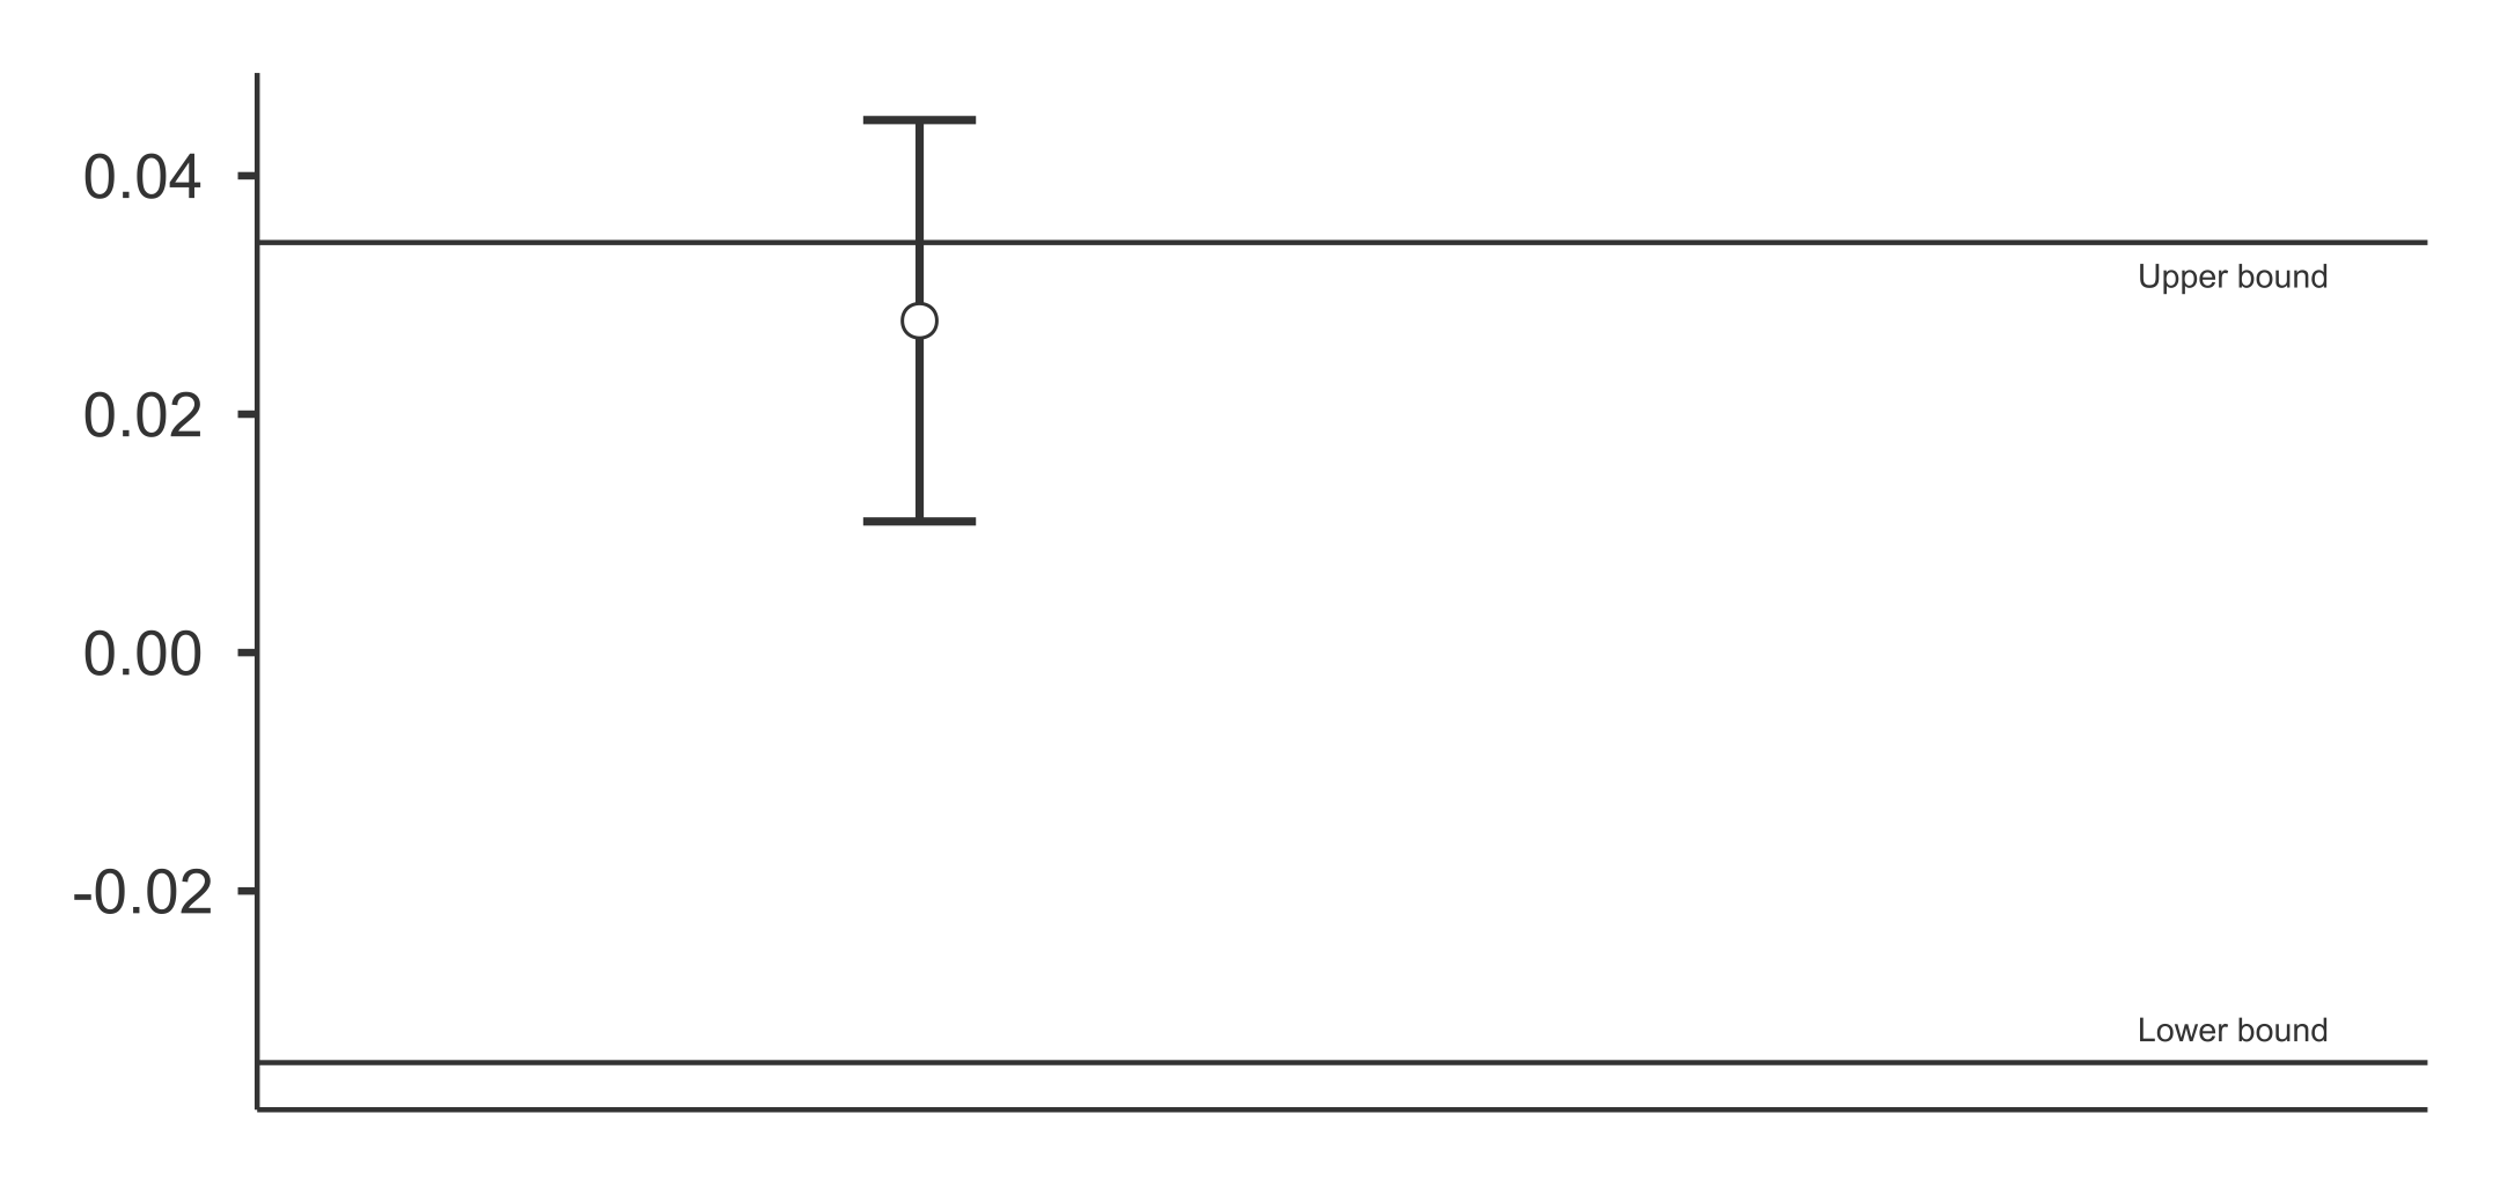
\includegraphics[width=\linewidth]{media/supplement/images-1.jpeg}
\end{table}

% \begin{figure}[h]

%   \caption{}
%   \label{}


% \end{figure}


















\begin{table}

  \caption{Linear regression with difference in pre-post reliability rating of manipulative messaging as the dependent variable }
  \label{tab:tableS33}


  \begin{tabularx}{\linewidth}{@{} X  S  S  S@{}}

    \toprule
    \emph{Predictors}                                    & {\emph{Estimates}}                        & {\emph{\emph{CI}}} & {\emph{p}} \\
    \midrule
    (Intercept)                                          & -0.02                                     & -0.08 -- 0.03      & 0.436      \\
    Condition [Treatment]                                & 0.00                                      & -0.01 -- 0.02      & 0.633      \\
    Gender [2]                                           & -0.01                                     & -0.02 -- 0.00      & 0.186      \\
    Gender [3]                                           & -0.03                                     & -0.06 -- 0.00      & 0.069      \\
    Grad [1]                                             & -0.00                                     & -0.01 -- 0.01      & 0.955      \\
    Age25-34                                             & -0.00                                     & -0.02 -- 0.01      & 0.580      \\
    Age35-44                                             & 0.01                                      & -0.02 -- 0.03      & 0.542      \\
    Age45-54                                             & -0.03                                     & -0.08 -- 0.01      & 0.130      \\
    Age [55 and over]                                    & 0.00                                      & -0.09 -- 0.10      & 0.964      \\
    Pol\_interest\_1                                     & -0.00                                     & -0.01 -- 0.01      & 0.973      \\
    LR\_Score                                            & -0.00                                     & -0.01 -- 0.01      & 0.906      \\
    FromMP [1]                                           & 0.01                                      & -0.01 -- 0.02      & 0.517      \\
    Lib\_Auth                                            & 0.01                                      & -0.00 -- 0.03      & 0.054      \\
    WAUse\_1                                             & -0.01                                     & -0.01 -- 0.00      & 0.198      \\
    News.checking\_1                                     & 0.01                                      & -0.00 -- 0.01      & 0.087      \\
    Social.checking\_1                                   & -0.00                                     & -0.01 -- 0.00      & 0.527      \\
    \midrule
    Observations                                         & \multicolumn{3}{@{} c @{}}{662}                                             \\
    R\textsuperscript{2} / R\textsuperscript{2} adjusted & \multicolumn{3}{@{} c @{}}{0.026 / 0.003}                                   \\
    \bottomrule
  \end{tabularx}


\end{table}


\begin{table}

  \caption{Linear regression with difference in pre-post confidence rating of manipulative messaging as the dependent variable }
  \label{tab:tableS34}



  \begin{tabularx}{\linewidth}{@{} X  S  S[table-space-text-post=\,\%]<{\,\%}
    r @{}}

    \toprule
    \emph{Predictors}                                    & {\emph{Estimates}}                         & {\emph{\emph{CI}}} & {\emph{p}}     \\
    \midrule
    (Intercept)                                          & -0.01                                      & -0.07 -- 0.05      & 0.783          \\
    Condition [Treatment]                                & -0.01                                      & -0.02 -- 0.01      & 0.335          \\
    Gender [2]                                           & -0.00                                      & -0.02 -- 0.01      & 0.570          \\
    Gender [3]                                           & -0.01                                      & -0.04 -- 0.02      & 0.622          \\
    Grad [1]                                             & -0.01                                      & -0.02 -- 0.01      & 0.218          \\
    Age25-34                                             & -0.01                                      & -0.02 -- 0.01      & 0.492          \\
    Age35-44                                             & -0.01                                      & -0.03 -- 0.02      & 0.603          \\
    Age45-54                                             & -0.04                                      & -0.08 -- 0.01      & 0.103          \\
    Age [55 and over]                                    & 0.00                                       & -0.10 -- 0.10      & 0.944          \\
    Pol\_interest\_1                                     & -0.00                                      & -0.01 -- 0.00      & 0.421          \\
    LR\_Score                                            & -0.01                                      & -0.02 -- 0.00      & 0.310          \\
    FromMP [1]                                           & -0.01                                      & -0.02 -- 0.01      & 0.523          \\
    Lib\_Auth                                            & 0.01                                       & -0.01 -- 0.02      & 0.253          \\
    WAUse\_1                                             & 0.00                                       & -0.01 -- 0.01      & 0.611          \\
    News.checking\_1                                     & 0.01                                       & 0.00 -- 0.02       & \textbf{0.032} \\
    Social.checking\_1                                   & -0.00                                      & -0.01 -- 0.00      & 0.203          \\
    \midrule
    Observations                                         & \multicolumn{3}{@{} c @{}}{662}                                                  \\
    R\textsuperscript{2} / R\textsuperscript{2} adjusted & \multicolumn{3}{@{} c @{}}{0.019 / -0.003}                                       \\
    \bottomrule
  \end{tabularx}


\end{table}








\begin{table}

  \caption{Linear regression with difference in pre-post sharing rating of manipulative messaging as the dependent variable }
  \label{tab:tableS35}


  \begin{tabularx}{\linewidth}{@{} X  S  S  S@{}}

    \toprule
    \emph{Predictors}                                    & {\emph{Estimates}}                         & {\emph{\emph{CI}}} & {\emph{p}} \\
    \midrule
    (Intercept)                                          & 0.04                                       & -0.02 -- 0.10      & 0.192      \\
    Condition [Treatment]                                & -0.01                                      & -0.02 -- 0.01      & 0.382      \\
    Gender [2]                                           & -0.00                                      & -0.02 -- 0.01      & 0.719      \\
    Gender [3]                                           & 0.00                                       & -0.03 -- 0.03      & 0.966      \\
    Grad [1]                                             & -0.00                                      & -0.02 -- 0.01      & 0.679      \\
    Age25-34                                             & 0.00                                       & -0.01 -- 0.02      & 0.603      \\
    Age35-44                                             & 0.00                                       & -0.02 -- 0.03      & 0.779      \\
    Age45-54                                             & -0.01                                      & -0.06 -- 0.03      & 0.628      \\
    Age [55 and over]                                    & -0.02                                      & -0.12 -- 0.09      & 0.746      \\
    Pol\_interest\_1                                     & -0.01                                      & -0.01 -- 0.00      & 0.059      \\
    LR\_Score                                            & -0.00                                      & -0.01 -- 0.01      & 0.434      \\
    FromMP [1]                                           & -0.00                                      & -0.02 -- 0.02      & 0.935      \\
    Lib\_Auth                                            & -0.00                                      & -0.02 -- 0.01      & 0.743      \\
    WAUse\_1                                             & -0.00                                      & -0.01 -- 0.00      & 0.314      \\
    News.checking\_1                                     & 0.01                                       & -0.00 -- 0.02      & 0.102      \\
    Social.checking\_1                                   & -0.00                                      & -0.01 -- 0.00      & 0.555      \\

    \midrule
    Observations                                         & \multicolumn{3}{@{} c @{}}{662}                                              \\
    R\textsuperscript{2} / R\textsuperscript{2} adjusted & \multicolumn{3}{@{} c @{}}{0.012 / -0.011}                                   \\
    \bottomrule
  \end{tabularx}


\end{table}
\begin{table}

  \caption{ANCOVA on Post-Treatment scores of reliability assessments (of manipulative items) -- data filtered for treatment participants that inputted the game password correctly}
  \label{tab:tableS36}


  \begin{tabularx}{\linewidth}{@{} l  S  S  S  S  S  S  c @{}}

    \toprule
    {Predictor} & {SumofSquares} & {\emph{df}} & {MeanSquare} & {\emph{F}} & {\emph{p}}       & {\textsubscript{partial }η\textsuperscript{2}} & \begin{tabular}{@{}c@{}}\textsubscript{partial }η\textsuperscript{2 }\\ 90\%\emph{CI}\\ {[}LL, UL{]}\end{tabular} \\
    \midrule
    (Intercept) & 0.17           & 1           & 0.17         & 23.97      & \emph{p} < 0.001 &                                                &                                                                                                                   \\
    F\_Rel\_Pre & 4.18           & 1           & 4.18         & 586.29     & \emph{p} < 0.001 & .56                                            & [.52, .60]                                                                                                        \\
    Condition   & 0.00           & 1           & 0.00         & 0.10       & .752             & .00                                            & [.00, .01]                                                                                                        \\
    Error       & 3.25           & 456         & 0.01         &            &                  &                                                &                                                                                                                   \\
    \bottomrule
  \end{tabularx}
  \emph{Note.} LL and UL represent the lower-limit and upper-limit of the partial η\textsuperscript{2} confidence interval, respectively.


\end{table}



\begin{table}

  \caption{ANCOVA on Post-Treatment scores of confidence in assessments (of manipulative items) -- data filtered for treatment participants that inputted the game password correctly}
  \label{tab:tableS37}


  \begin{tabularx}{\linewidth}{@{} l  S  S  S  S  S  S  c @{}}
    \toprule
    {Predictor}  & {SumofSquares} & {\emph{df}} & {MeanSquare} & {\emph{F}} & {\emph{p}}       & {\textsubscript{partial }η\textsuperscript{2}} & \begin{tabular}{@{}c@{}}\textsubscript{partial }η\textsuperscript{2 }\\ 90\%\emph{CI}\\ {[}LL, UL{]} \end{tabular} \\
    \midrule
    (Intercept)  & 0.55           & 1           & 0.55         & 70.67      & \emph{p} < 0.001 &                                                &                                                                                                                    \\
    F\_Conf\_Pre & 3.54           & 1           & 3.54         & 458.50     & \emph{p} < 0.001 & .50                                            & [.45, .54]                                                                                                         \\
    Condition    & 0.00           & 1           & 0.00         & 0.25       & .615             & .00                                            & [.00, .01]                                                                                                         \\
    Error        & 3.52           & 456         & 0.01         &            &                  &                                                &                                                                                                                    \\
    \bottomrule
  \end{tabularx}

  \emph{Note.} LL and UL represent the lower-limit and upper-limit of the partial η\textsuperscript{2} confidence interval, respectively.

\end{table}



\begin{table}

  \caption{ANCOVA on Post-Treatment scores of sharing measure (of manipulative items) -- data filtered for treatment participants that inputted the game password correctly}
  \label{tab:tableS38}


  \begin{tabularx}{\linewidth}{@{} l  S  S  S  S  S  S  c @{}}
    \toprule
    {Predictor}   & {SumofSquares} & {\emph{df}} & {MeanSquare} & {\emph{F}} & {\emph{p}}       & {\textsubscript{partial }η\textsuperscript{2}} & \begin{tabular}{@{}c@{}}\textsubscript{partial }η\textsuperscript{2 }\\ 90\%\emph{CI}\\ {[}LL, UL{]} \end{tabular} \\
    \midrule
    (Intercept)   & 0.32           & 1           & 0.32         & 42.52      & \emph{p} < 0.001 &                                                &                                                                                                                    \\
    F\_Share\_Pre & 4.85           & 1           & 4.85         & 652.45     & \emph{p} < 0.001 & .59                                            & [.54, .63]                                                                                                         \\
    Condition     & 0.00           & 1           & 0.00         & 0.67       & .413             & .00                                            & [.00, .01]                                                                                                         \\
    Error         & 3.39           & 456         & 0.01         &            &                  &                                                &                                                                                                                    \\
    \bottomrule
  \end{tabularx}

  \emph{Note.} LL and UL represent the lower-limit and upper-limit of the partial η\textsuperscript{2} confidence interval, respectively.

\end{table}





\begin{table}

  \caption{Proportion of rural population across participants' states }
  \label{tab:tableS39}


  \begin{tabularx}{\linewidth}{@{} X  r  r  r@{}}



    \toprule
    \emph{State}   & \emph{n} & \emph{Rural population (\%)} & \emph{Weighted Rural}\textsuperscript{\emph{1}} \\

    \midrule
    Bihar          & 19       & 89                           & 1685                                            \\
    Chhattisgarh   & 42       & 77                           & 3226                                            \\
    Delhi          & 3        & 2                            & 8                                               \\
    Haryana        & 5        & 65                           & 325                                             \\
    Jharkhand      & 26       & 76                           & 1976                                            \\
    Madhya Pradesh & 471      & 72                           & 34100                                           \\
    Rajasthan      & 120      & 75                           & 9012                                            \\
    Unknown*       & 6        & 69                           & 413                                             \\
    Uttar Pradesh  & 33       & 78                           & 2564                                            \\
                   &          & \textbf{Weighted Mean}       & 73.5                                            \\
  \end{tabularx}

  *\emph{For missing values, rural proportion of India's national population was imputed }

  \textsuperscript{\emph{1}}\emph{Weighted Rural = n * Rural population (\%)}

  \emph{All rural population (\%) values sourced from: }\emph{ }

\end{table}



\begin{table}

  \caption{Distribution between conditions by state}
  \label{tab:tableS40}


  \begin{tabularx}{\linewidth}{@{} X  l  r@{}}

    \toprule
    \emph{Condition} & \emph{State}   & \emph{n} \\
    \midrule
    Control          & Bihar          & 15       \\
    Treatment        & Bihar          & 4        \\
    Control          & Chhattisgarh   & 22       \\
    Treatment        & Chhattisgarh   & 20       \\
    Control          & Delhi          & 1        \\
    Treatment        & Delhi          & 2        \\
    Control          & Haryana        & 5        \\
    Control          & Jharkhand      & 10       \\
    Treatment        & Jharkhand      & 16       \\
    Control          & Madhya Pradesh & 232      \\
    Treatment        & Madhya Pradesh & 239      \\
    Control          & Rajasthan      & 62       \\
    Treatment        & Rajasthan      & 58       \\
    Control          & Unknown        & 4        \\
    Treatment        & Unknown        & 2        \\
    Control          & Uttar Pradesh  & 14       \\
    Treatment        & Uttar Pradesh  & 19       \\
    \bottomrule
  \end{tabularx}


\end{table}
\clearpage



\begin{figure}[h!]

  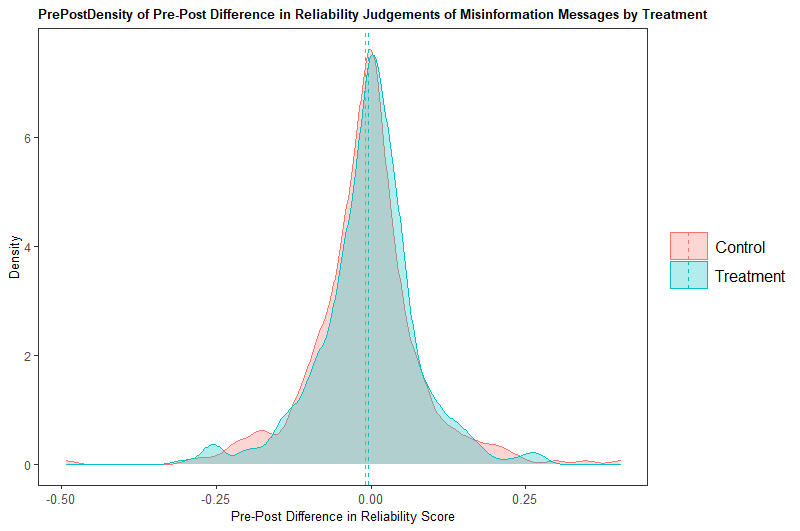
\includegraphics[width=\linewidth]{media/supplement/images1.jpeg}
  \caption{Distribution of Pre-Post Differences in Reliability Judgements of Manipulative Items by Condition}
  \label{fig:figS1}
\end{figure}




\begin{figure}[h!]

  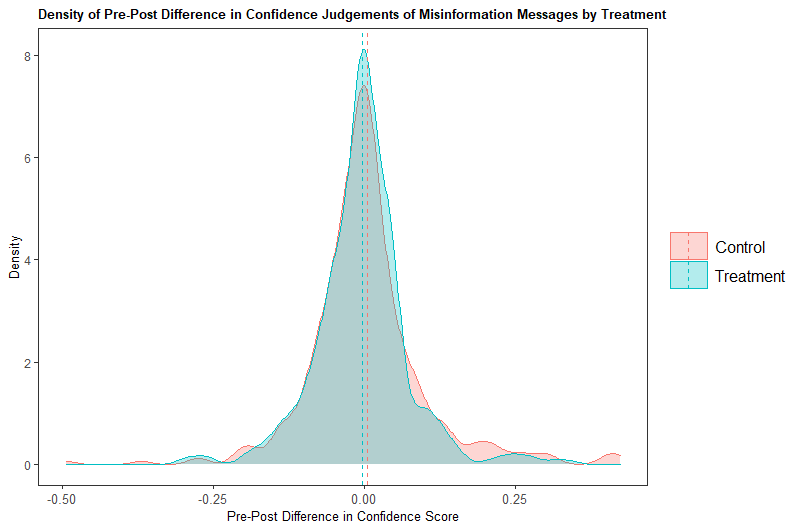
\includegraphics[width=\linewidth]{media/supplement/images2.jpeg}
  \caption{Distribution of Pre-Post Differences in Confidence in Judgements of Manipulative Items by Condition}
  \label{fig:figS2}


\end{figure}




\begin{figure}[h]

  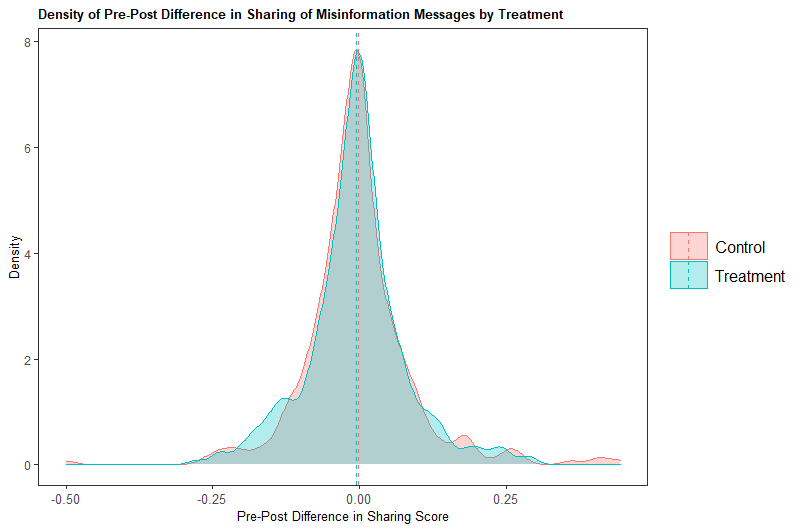
\includegraphics[width=\linewidth]{media/supplement/images3.jpeg}
  \caption{Distribution of Pre-Post Differences in Likelihood to Share Manipulative Items by Condition}
  \label{}


\end{figure}






\begin{figure}

  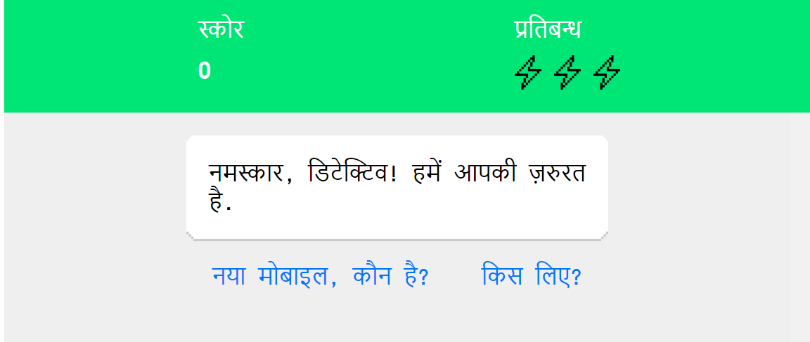
\includegraphics[width=\linewidth]{media/supplement/images4.jpeg}
  \caption{In-game Screenshot - First screen shown after starting the game, introducing the
    character and motive \\
    Translation: \\
    Green Bar (Left to Right): “Score” “Sanctions” \\
    White Box: “Hello, Detective! We need you”}
  \label{}


\end{figure}



\begin{figure}

  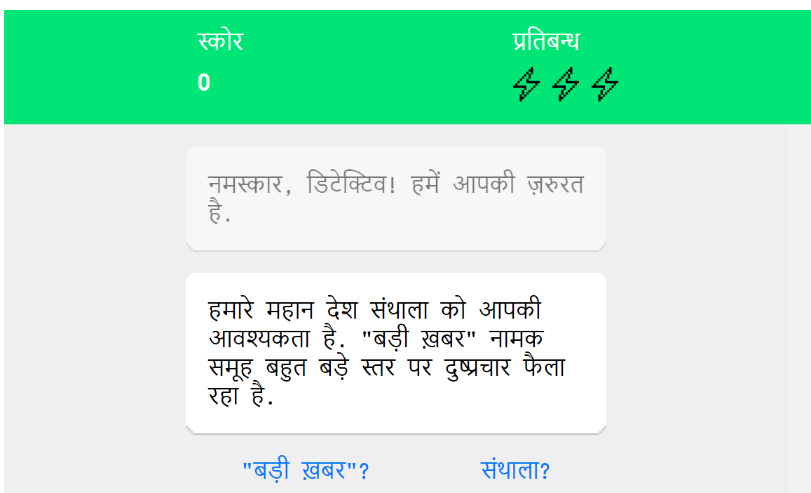
\includegraphics[width=\linewidth]{media/supplement/images5.jpeg}

  \caption{In-game Screenshot - Second screen shown after starting the game, depicting an explanation of the propaganda spreading on \mbox{WhatsApp}.\\ Translation: \\
    \emph{Green Bar (Left to Right): “Score” “Sanctions”} \\
    \emph{White Box: “Our great country Santhala needs you. }\emph{A group called “Big News” is spreading propaganda at a very large scale”} \\
    \emph{Blue Text (Left to Right): “New mobile, who's this?” “For what?”} \\
    \emph{Blue text: “Big News?” “Santhala?”}
  }

  \label{}


\end{figure}




\begin{figure}

  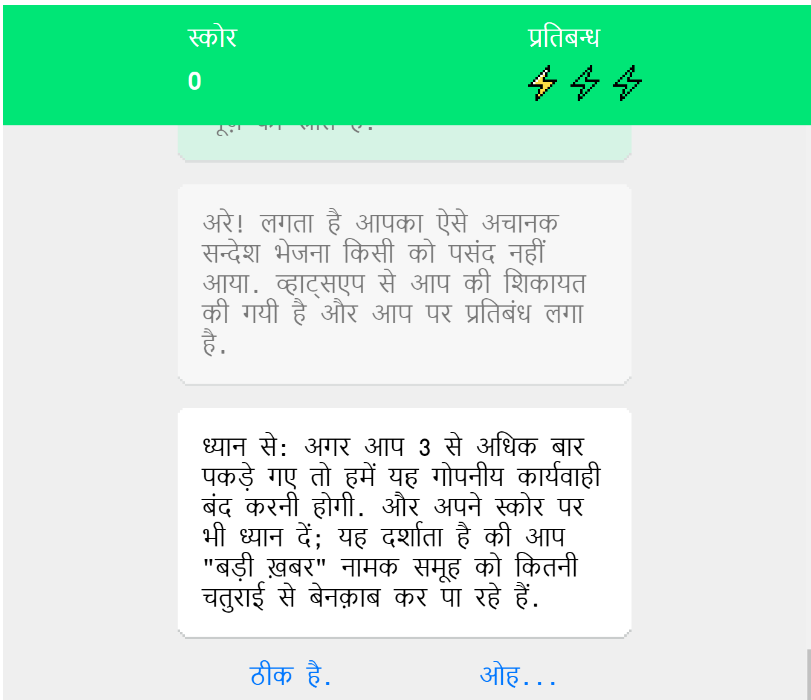
\includegraphics[width=\linewidth]{media/supplement/images6.jpeg}

  \caption{In-game Screenshot - An in-game screenshot explaining the rules of the game. \\
    Translation: \\
    \emph{Green Bar (Left to Right): “Score” “Sanctions”} \\
    \emph{White Box: “Be careful: If you get caught more than 3 times then we have to stop this secrecy. }\emph{And watch your score as well; this will tell you how much you are exposing the “Bad News” group.”} \\
    \emph{Blue text: “That's fine”}\emph{}\emph{“Okay…”}
  }
  \label{}


\end{figure}












\clearpage



\begin{figure}

  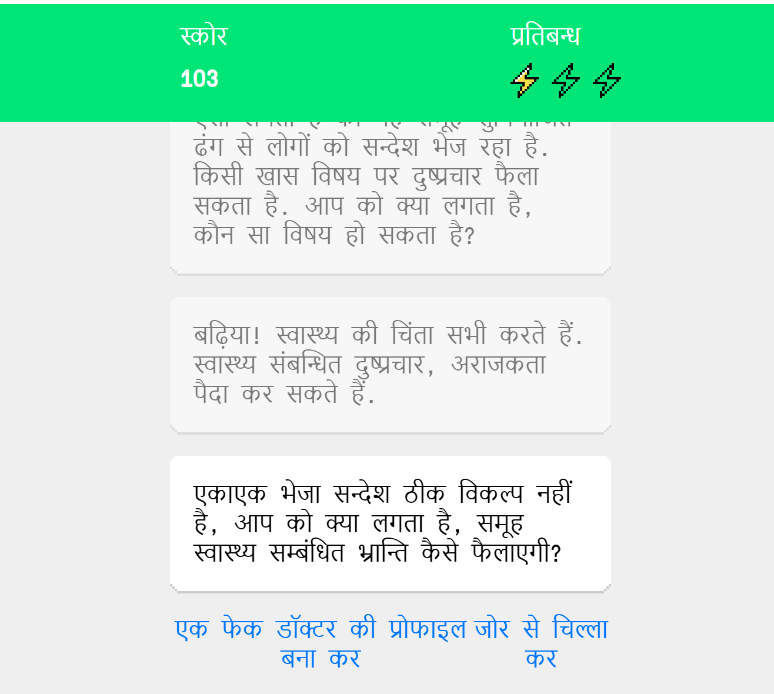
\includegraphics[width=\linewidth]{media/supplement/images7.jpeg}
  \caption{In-game screenshot - Showing how a Fake News technique (using a fake expert) is taught.
    Translation:
    \emph{Green Bar (Left to Right): “Score” “Sanctions”}\\
    \emph{White Box: “Just sending a message all of a sudden isn't the right way, what do you think, how will the group spread this health-related misconception?”}\\
    \emph{Blue text: “By creating a fake doctor profile”} {“By shouting loudly”}}
  \label{fig:figS7}
\end{figure}

\clearpage



\begin{figure}
  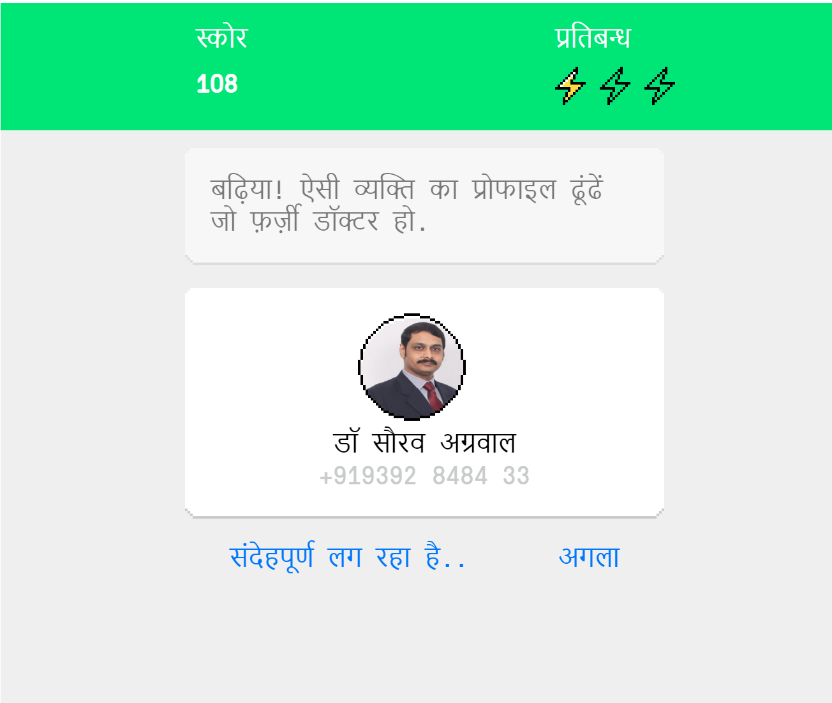
\includegraphics[width=\linewidth]{media/supplement/images8.jpeg}
  \caption{
    In-game screenshot showing how the Fake News techniques is taught. Continuation of Figure S7.
    Translation:\\
    \emph{Green Bar (Left to Right): “Score” “Sanctions”}\\
    \emph{Grey Box: “Well done! }\emph{Find the profile of a person who is a fake doctor”}\\
    \emph{White Box: “Dr Saurav Agrawal}”\\
    \emph{Blue Text: “It looks suspicious…” “Next”}\\
  }
  \label{fig:figS8}
\end{figure}







\begin{figure}

  \centering
  
\includegraphics[height=.5\textheight]{media/supplement/images9a.jpeg}
  
\includegraphics[height=.5\textheight]{media/supplement/images9b.jpeg}
  \caption{Example of a translated manipulative \mbox{WhatsApp} prompt (with English version from another study) intended to show the use of a fake expert. \\ Screenshot reads: “Hello! \\ Nowadays it's been very dry. \\ Even in the rainy season, it does not rain”, “Not sure what's happening with the weather these days. \\ Maybe this is happening because of the climate change in the environment”,\\ “Do you think this is happening because of climate change?”,\\ “I'm not sure, it's difficult to say, farming has become very difficult”,\\ “Hello, I am a scientist, climate change is a big reason for whatever is happening in our environment. \\ We have to save our environment.”,\\ “Right, interesting”.}
  \label{}
\end{figure}


\end{document}